\documentclass[12pt,a4paper,openright,twoside]{book}
\usepackage[utf8]{inputenc}
\usepackage{disi-thesis}
\usepackage{code-lstlistings}
\usepackage{notes}
\usepackage{shortcuts}
\usepackage{acronym}

\school{\unibo}
\programme{Corso di Laurea Magistrale in Ingegneria e Scienze Informatiche}
\title{Fancy Title}
\author{Cecilia Teodorani}
\date{\today}
\subject{Project Management}
\supervisor{Prof. Marco Antonio Boschetti}
\cosupervisor{Dott. Mirco Mattarozzi}
\session{IV}
\academicyear{2023-2024}

% Definition of acronyms
\acrodef{ESI}{Enterprise Service Infrastructure}
\acrodef{SBS}{Smart Business Solutions}
\acrodef{ERP}{Enterprise Resource Planning}
\acrodef{PBC}{Packaged Business Capabilities}
\acrodef{PAM}{Peer Network Activity Management}
\acrodef{PMBOK}{Project Management Body of Knowledge}
\acrodef{WBS}{Work Breakdown Structure}

\mainlinespacing{1.241} % line spacing in mainmatter, comment to default (1)

\begin{document}

\frontmatter\frontispiece

\begin{abstract}	
    %Very brief (e.g. 250-300 words)
    %Context, Problem/Objectives, Methods/Contribution, Results, Conclusions

Il presente lavoro nasce dall’esigenza di \textit{Peer Network} di ottimizzare la gestione
dei progetti aziendali. L’azienda opera nel settore della digitalizzazione e re-ingegnerizzazione
dei processi per i propri clienti, sviluppando applicazioni componibili anziché software interamente
personalizzati. Ogni entità di business coinvolta viene implementata come un'unità modulare,
denominata \acl{PBC}, che integra sia i propri dati che le azioni eseguibili su di essa. Oltre a
realizzare soluzioni per i clienti con questo approccio, \textit{Peer Network} sviluppa internamente
nuove \acl{PBC} e un’applicazione gestionale interna, \acl{PAM}, volta a migliorare l’efficienza
delle attività amministrative e organizzative.

L’analisi è iniziata esaminando nel dettaglio tutte le fasi del ciclo di vita di un progetto, dalle
attività gestionali e operative iniziali, fino all’installazione del sistema e alla fase di supporto.
Successivamente, partendo dai principi teorici del \acl{PMBOK}, dall’esperienza maturata in altri contesti
lavorativi e considerando la necessità di non poter stravolgere il metodo di lavoro aziendale, sono state
proposte soluzioni pratiche per rendere più efficiente la gestione dei progetti.

Una delle soluzioni concretamente implementate in \acl{PAM} durante questo lavoro riguarda l’automazione
dell’inserimento e dell’aggiornamento dei dati economici di ciascun progetto, inclusi costi, ricavi e
margini, sia pianificati che effettivi. In precedenza, questa gestione avveniva manualmente tramite
fogli elettronici, con un dispendio di tempo e un maggior rischio di errore. L’integrazione in \acl{PAM}
consente invece di ridurre i tempi di compilazione, centralizzare i dati in un’unica piattaforma e migliorare
l'affidabilità delle informazioni grazie all’automazione di alcuni inserimenti e calcoli.

\end{abstract}

\begin{dedication} % this is optional
Optional. Max a few lines.
\end{dedication}

%----------------------------------------------------------------------------------------
\tableofcontents   
%\listoffigures     % (optional) comment if empty
%\lstlistoflistings % (optional) comment if empty
%----------------------------------------------------------------------------------------

\mainmatter

\chapter{Introduction}
\label{chap:introduction}

Write your intro here.
\sidenote{Add sidenotes in this way. They are named after the author of the thesis}

You can use acronyms that your defined previously,
such as \ac{IoT}.
%
If you use acronyms twice,
they will be written in full only once
(indeed, you can mention the \ac{IoT} now without it being fully explained).
%
In some cases, you may need a plural form of the acronym.
%
For instance,
that you are discussing \acp{vm},
you may need both \ac{vm} and \acp{vm}.

\paragraph{Structure of the Thesis}

\note{At the end, describe the structure of the paper}


\chapter{Progetto}
\label{chap:project}

\textit{Peer Network} supporta le aziende nella revisione e reingegnerizzazione dei processi aziendali, adottando un
approccio basato su \textbf{processi componibili}, un esempio è presente in \Cref{fig:composable-process}. Questo approccio
supera i limiti dei sistemi monolitici tradizionali, introducendo moduli autonomi, riutilizzabili e facilmente
combinabili, che garantiscono flessibilità e adattabilità di fronte ai cambiamenti operativi.

\begin{figure}
    \centering
    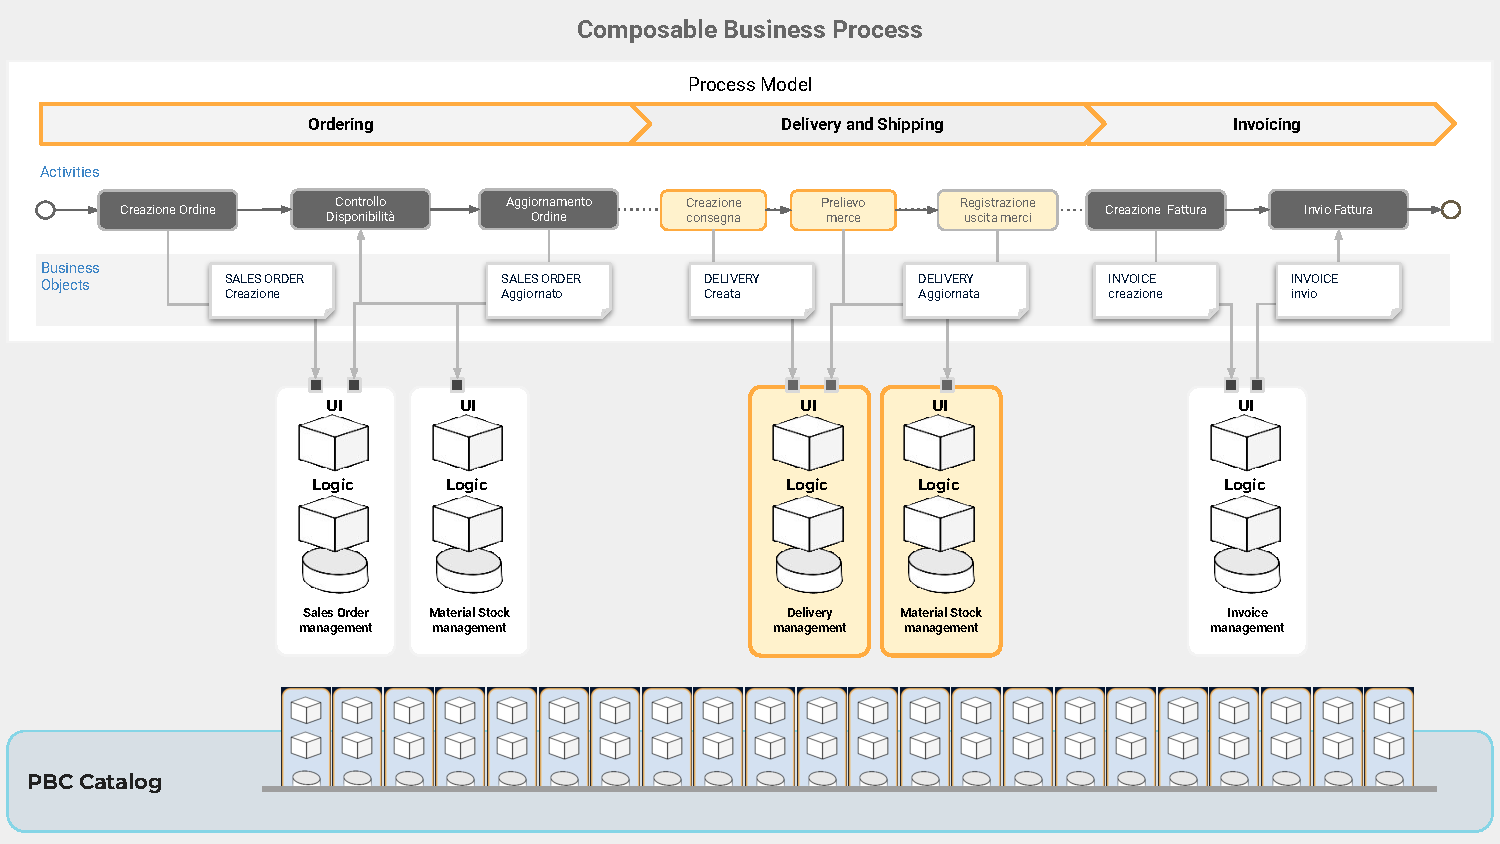
\includegraphics[width=\linewidth]{figures/composable_process.pdf}
    \caption{Struttura di un processo componibile}
    \label{fig:composable-process}
\end{figure}

La ridefinizione dei processi inizia identificando le attività da svolgere e gli \textbf{oggetti di business (BO)} coinvolti.
Gli oggetti di business rappresentano elementi chiave di un’organizzazione all’interno di un sistema informativo. Essi
riflettono entità reali, ad esempio cliente, prodotto, ordine, consegna, includendo ciascuno attributi specifici
(es. nell’ordine ci sono numero ordine, stato, riferimento ai prodotti). Questi oggetti, modellati in modo chiaro,
facilitano la gestione e l’integrazione dei processi aziendali, fungendo da base per la progettazione delle \ac{PBC}.

Per analizzare e modellare questi elementi, viene applicato il \textbf{Domain Driven Design}\cite{evans2004domain}, un metodo che consente di
suddividere il dominio aziendale in \textbf{Bounded Contexts} distinti. Ogni contesto rappresenta un sottoinsieme indipendente
e ben definito del dominio, facilitando la gestione e l’organizzazione dei processi.

All’interno di ciascun Bounded Context, gli oggetti di business vengono implementati come \textbf{\ac{PBC}}.
Queste unità modulari e riutilizzabili rappresentano specifiche entità aziendali che racchiudono in sé i dati e le azioni che
si possono compiere su di esse in un formato indipendente e facilmente integrabile. Come schematizzato nella \Cref{fig:pbc-struttura}
e nell’esempio in \Cref{fig:composable-process}, ciascuna \ac{PBC} descritta nelle ricerche di \textit{Gartner}\cite{natis2019innovation}\cite{burke2020top} include:

\begin{itemize}
    \item una \textbf{struttura dati} per rappresentare le informazioni associate alla \ac{PBC},
    \item un insieme di \textbf{API} di base per eseguire azioni sincrone sull'oggetto,
    \item un insieme di \textbf{eventi} di base per l'integrazione asincrona,
    \item una o più \textbf{interfacce utente} (opzionale).
\end{itemize}

\begin{figure}
    \centering
    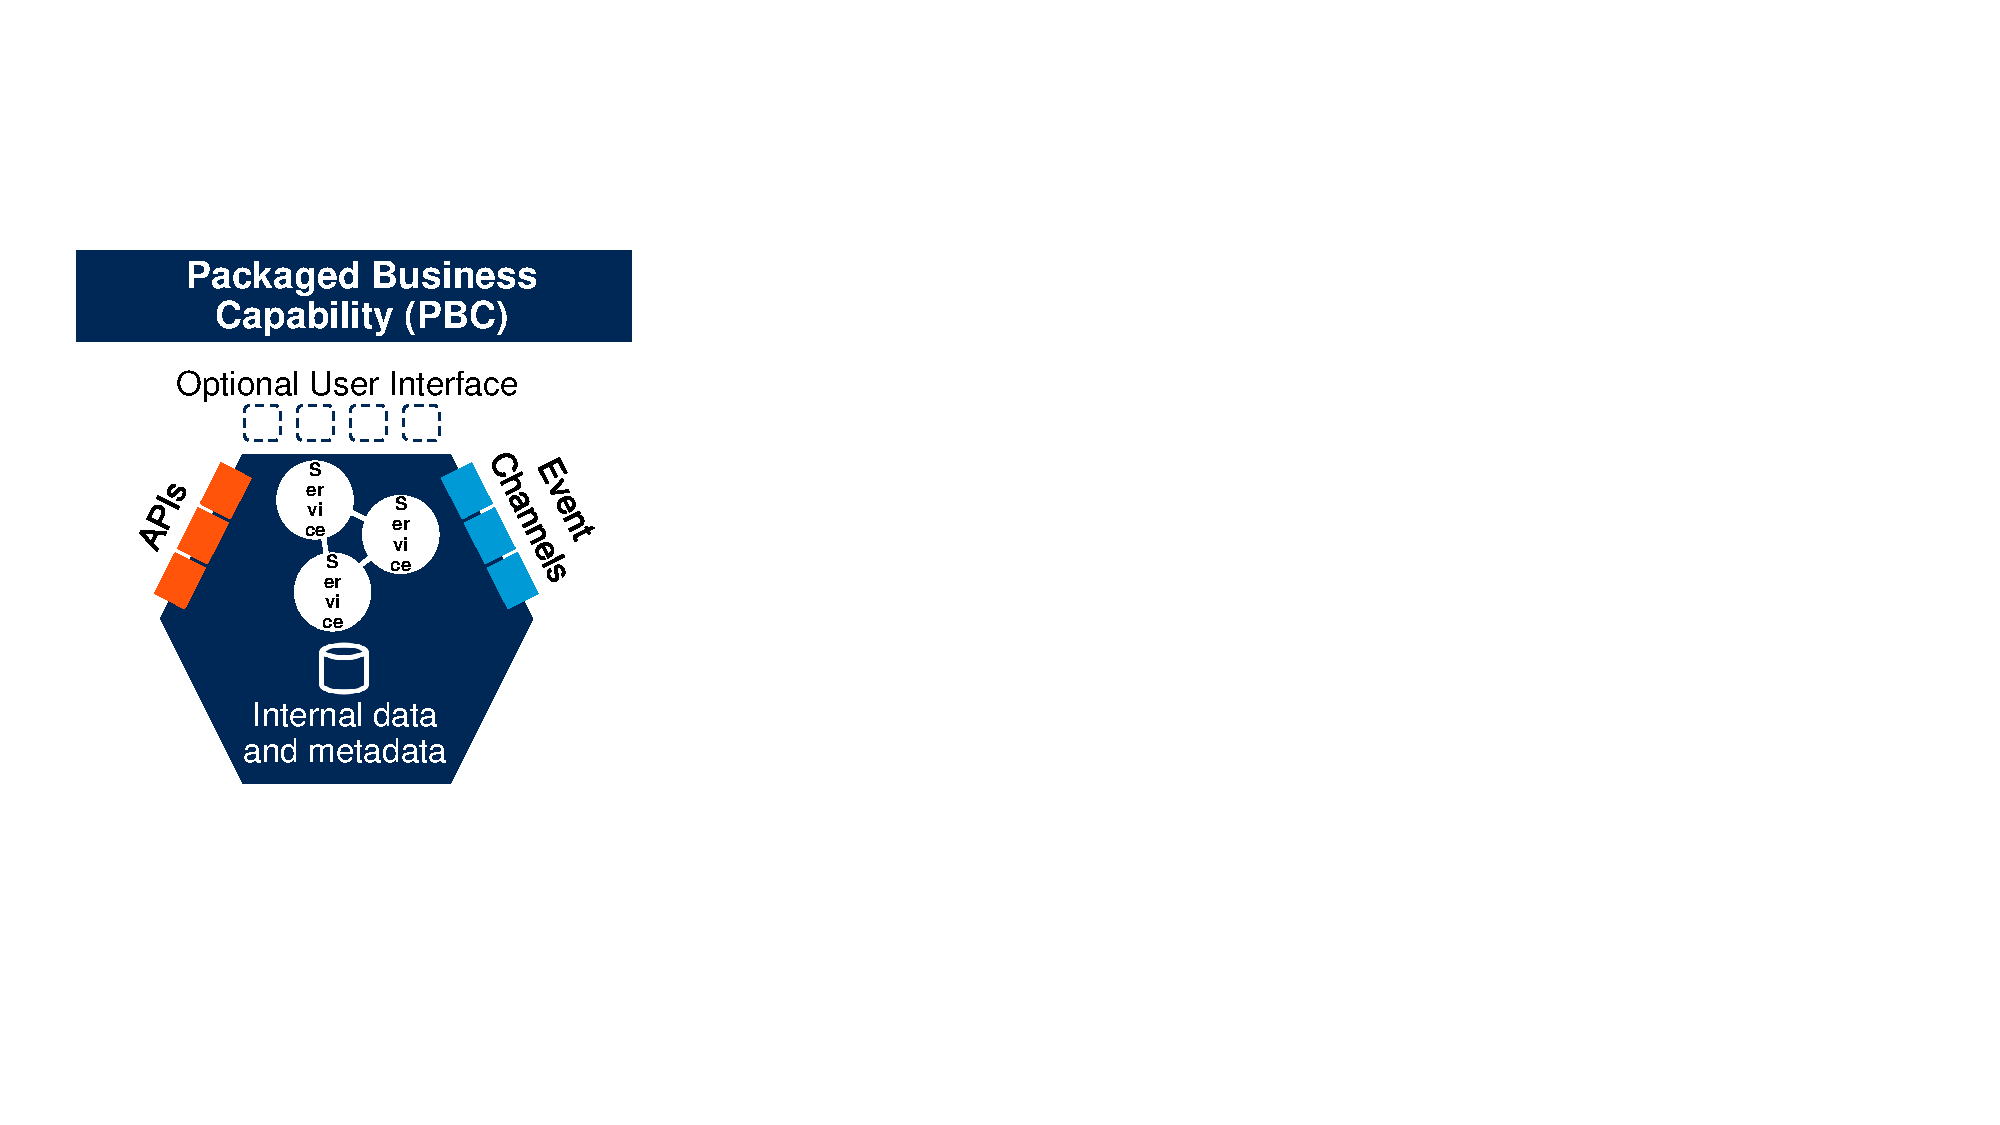
\includegraphics[scale=0.6]{figures/PBCstructure.pdf}
    \caption{Struttura \ac{PBC} secondo \textit{Gartner}}
    \label{fig:pbc-struttura}
\end{figure}

Questa struttura consente di progettare \textbf{applicazioni componibili}, assemblate combinando \ac{PBC} esistenti o sviluppandone di nuove.
Secondo \textit{Gartner}, tale approccio accelera il time-to-market, migliora l’adattabilità ai cambiamenti e garantisce soluzioni coerenti
con le esigenze operative dei clienti. Le applicazioni componibili sono progettate per richiamare dinamicamente i servizi dei
sistemi sottostanti, adottando un modello di integrazione process-centric, dove i processi di business guidano l’organizzazione
anziché i dati o le singole applicazioni. Questo tipo di applicazioni hanno una struttura che distingue chiaramente due livelli:

\begin{itemize}
    \item \textbf{frontend}, focalizzato sull’esperienza utente (UX) e costruito con interfacce intuitive,
    \item \textbf{backend}, dedicato alla logica applicativa, implementato tramite \ac{PBC} indipendenti.
\end{itemize}

Una delle caratteristiche distintive di \textit{Peer Network} è la capacità di trasferire su componenti di business, le \ac{PBC} appunto, le proprie
competenze di dominio e costruire con esse soluzioni componibili, invece di sviluppare software interamente personalizzati per ogni cliente.
Questo approccio è stato favorito dall’esperienza che l’azienda ha maturato in tanti anni di attività sulla piattaforma \ac{ERP} di
SAP\footnote{https://www.sap.com/italy/index.html}, che ha storicamente definito i principali standard internazionali nel settore.

Le soluzioni di \textit{Peer Network} semplificano il lavoro dei diversi attori di un processo di business, grazie a flussi operativi chiari e una
gestione meno complessa rispetto alle tradizionali piattaforme \ac{ERP}, come SAP. L'integrazione con la piattaforma \ac{ESI}, che funge anche da
repository per le \ac{PBC}, permette ai sistemi sviluppati di comunicare direttamente con gli \ac{ERP} aziendali. Questo processo non solo facilita
il recupero e l'elaborazione dei dati necessari, ma introduce anche una serie di funzionalità aggiuntive. Le informazioni così ottenute vengono
presentate attraverso interfacce grafiche progettate per ottimizzare usabilità ed efficienza operativa.

\section{Gestione Progetti}
Nel corso del tempo, nonostante gli sforzi per migliorare l’organizzazione e incrementare l’efficienza lavorativa, in \textit{Peer Network} sono
emerse difficoltà nel gestire contemporaneamente tutti i progetti. Questi ultimi si dividono in due principali categorie:

\begin{itemize}
    \item \textbf{progetti esterni}: soluzioni sviluppate per i clienti, denominate \ac{SBS},
    \item \textbf{progetti interni}, suddivisi ulteriormente in due tipologie:
        \begin{itemize}
            \item \textbf{ricerca e sviluppo}: attività principale è l'aggiornamento continuo delle \ac{PBC} per integrarle
            rapidamente nelle soluzioni destinate ai clienti e il conseguente miglioramento della piattaforma \ac{ESI};
            \item \textbf{software gestionale \ac{PAM}}: applicazione utilizzata internamente per il monitoraggio e la gestione del lavoro svolto dai dipendenti.
        \end{itemize}
\end{itemize}

Nel contesto di questa complessità operativa e dinamicità, i project manager e i dipendenti hanno individuato alcune problematiche generali.
La più evidente è la scarsità di personale rispetto al carico di lavoro, che porta gli sviluppatori a ricoprire più ruoli contemporaneamente,
sia all’interno dello stesso progetto sia su più progetti. Questo sovraccarico rende difficile per ciascuno svolgere al meglio i compiti assegnati.
Inoltre, i project manager, provenienti da un background tecnico, tendono ad adottare un approccio eccessivamente orientato agli aspetti tecnici,
trascurando l'analisi di dominio e la pianificazione strategica. Un ulteriore ostacolo è rappresentato dalla difficoltà nel delegare compiti: le
competenze sono concentrate in poche persone esperte e il coinvolgimento di risorse junior richiede tempo e sforzi per formazione e supervisione,
che spesso vengono percepiti come un rallentamento delle attività.

Per affrontare queste problematiche, l’azienda ha deciso di uniformare il più possibile la gestione dei progetti, adottando un approccio standardizzato
per l’intero ciclo di vita. Basandosi sui principi del \textbf{\ac{PMBOK}}\cite{project2021guide}, i project manager hanno quindi elaborato lo schema
del ciclo di vita ideale di un progetto in \textit{Peer Network}, riportato in \Cref{fig:fasi-progettuali}. Le future modifiche nella gestione dovranno
progressivamente allinearsi a questo modello.

Il ciclo di vita del progetto è stato suddiviso in tre fasi principali. La prima, denominata “Idea, Design, Economics”, prevede l’analisi iniziale di un
nuovo progetto, la progettazione, la definizione del budget e la stipula del contratto. La seconda fase “Progetto Software,” si concentra sull’analisi
approfondita dei requisiti, sulla pianificazione e sullo sviluppo, fino al rilascio del prodotto. La terza fase, “Supporto e Servizio,” riguarda l’assistenza
post-installazione e le attività di manutenzione correttiva per garantire il corretto funzionamento del sistema.

\begin{figure}
    \centering
    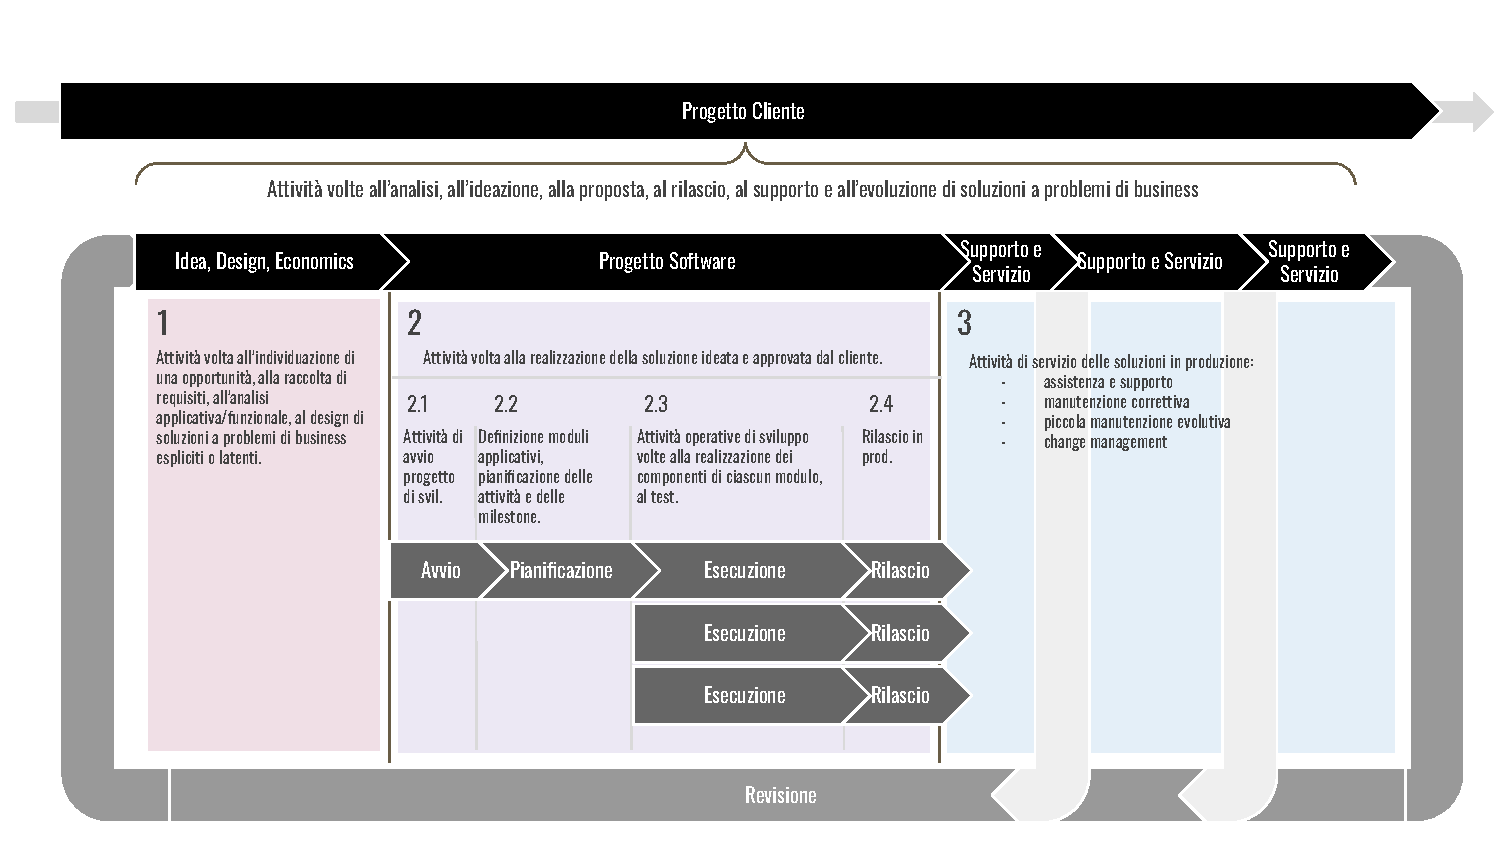
\includegraphics[width=\linewidth]{figures/FasiProgettualiPN.pdf}
    \caption{Ciclo di vita ideale per un progetto in \textit{Peer Network}}
    \label{fig:fasi-progettuali}
\end{figure}

Per raggiungere l'obiettivo di migliorare la gestione dei progetti, è innanzitutto fondamentale esaminare in dettaglio tutte le attività svolte nel novembre 2024,
identificando i problemi riscontrati dai dipendenti in ciascuna fase. Successivamente, basandosi sulle linee guida del \ac{PMBOK} e tenendo conto delle specifiche
esigenze aziendali, vengono proposti deliverables mirati, come schemi, analisi e documenti, per affrontare e risolvere le criticità emerse. Qualora alcune proposte
non risultassero applicabili per ragioni aziendali, vengono fornite spiegazioni che giustificano le decisioni adottate. Tutte queste informazioni vengono riportate
nel Capitolo \ref{chap:Contribution}.

\section{Peer Network Activity Management}
Il software interno \textbf{Peer Network Activity Management (PAM)} attualmente supporta l’amministrazione nella gestione delle risorse umane, nel monitoraggio e nella rendicontazione mensile
delle ore di lavoro dei dipendenti sui vari progetti, oltre a generare automaticamente report mensili da allegare alle fatture da inviare ai clienti.
Queste rappresentano le prime funzionalità implementate, considerate le più urgenti. Tuttavia, \ac{PAM} è stato concepito con una visione più ampia, mirata
alla gestione complessiva dell'azienda.

Per anni, il processo di fatturazione aziendale è stato gestito in modo poco strutturato e senza strumenti specifici, richiedendo circa due settimane
di lavoro mensile, oltre ad un contributo rilevante da parte dei project manager. Sebbene parzialmente automatizzato tramite il software Knime\footnote{https://www.knime.com},
il flusso di lavoro, illustrato in parte nella \Cref{fig:fatturazione-knime}, richiedeva una significativa supervisione manuale per avviare e monitorare ciascuna fase.
Inoltre, il processo prevedeva frequenti operazioni manuali di importazione ed esportazione di dati tramite diversi fogli elettronici Google
Sheet\footnote{https://workspace.google.com/intl/it/products/sheets/}.

\begin{figure}
    \centering
    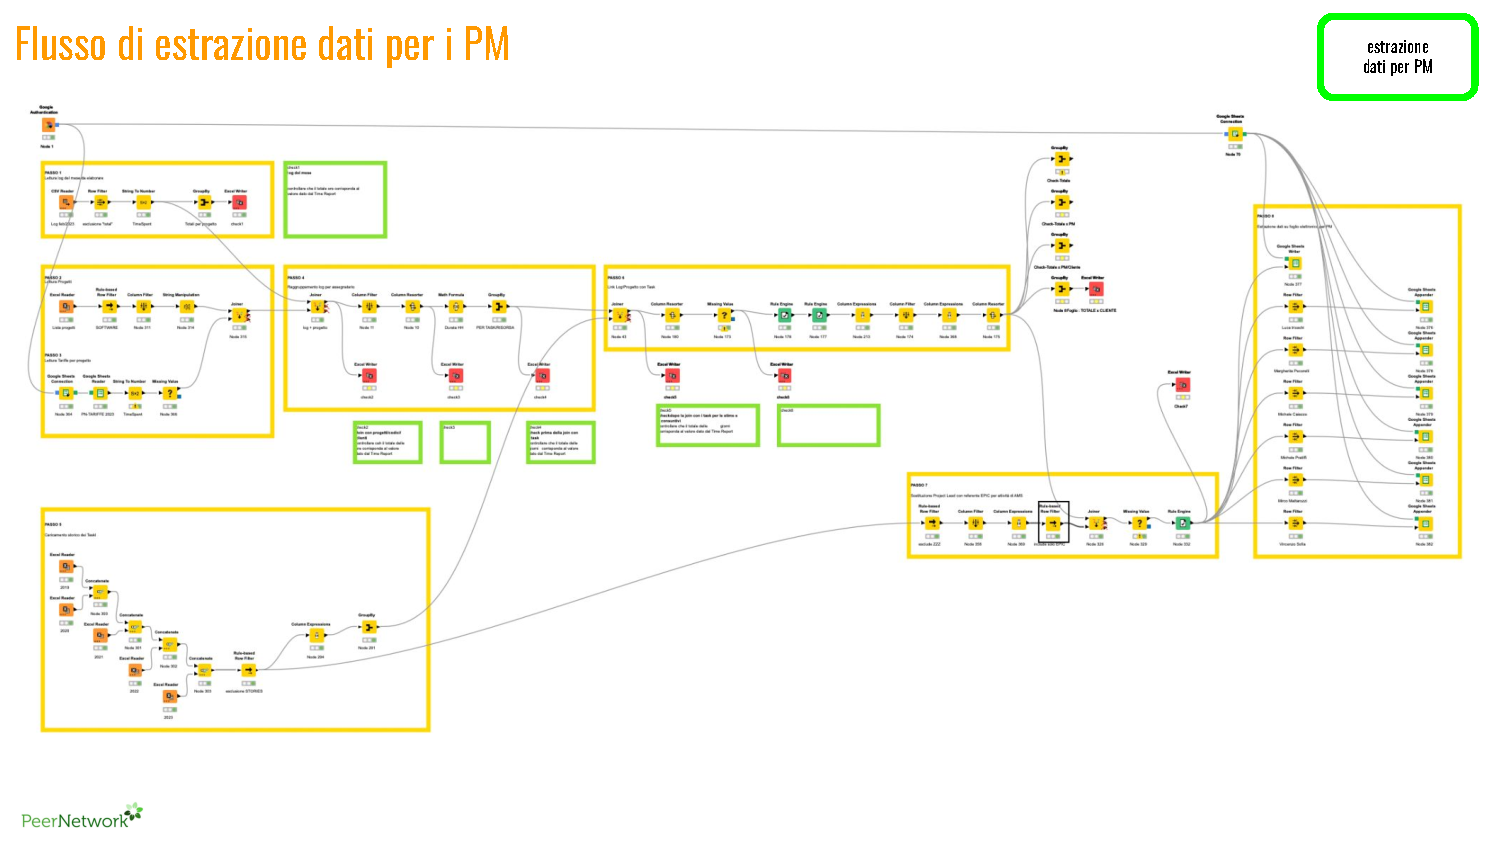
\includegraphics[width=\linewidth]{figures/FatturazioneKnime.pdf}
    \caption{Struttura su Knime riguardante una parte del processo di fatturazione, cioè l’estrazione di dati per i project manager}
    \label{fig:fatturazione-knime}
\end{figure}

Questo processo risultava troppo dispendioso in termini di tempo ed era basato su numerosi passaggi manuali. Per affrontare queste criticità, a gennaio 2024
è stato avviato il progetto interno \ac{PAM}, partendo con l’obiettivo di automatizzare gran parte del processo di fatturazione.
Le attività e il loro ordine di esecuzione sono schematizzate nella \Cref{fig:fatturazione}.

A partire da ottobre 2024, è stata resa disponibile la prima versione del sistema, che consente di completare l’intero flusso dal passaggio “estrazione dati
per PM” alla “generazione dei rapportini,” in poche ore anziché nelle circa due settimane precedentemente necessarie. L’utilizzo dei fogli elettronici da creare,
modificare o importare è stato completamente eliminato: l’intero processo è ora gestito dal gestionale, con l’utente che interagisce direttamente tramite un’unica
interfaccia grafica. L’automazione della fase di estrazione dati è stata resa possibile grazie all’integrazione con Jira\footnote{https://www.atlassian.com/software/jira},
uno strumento per la gestione e il monitoraggio dei progetti che consente ai dipendenti di registrare le ore lavorate su ciascun progetto.

\begin{figure}
    \centering
    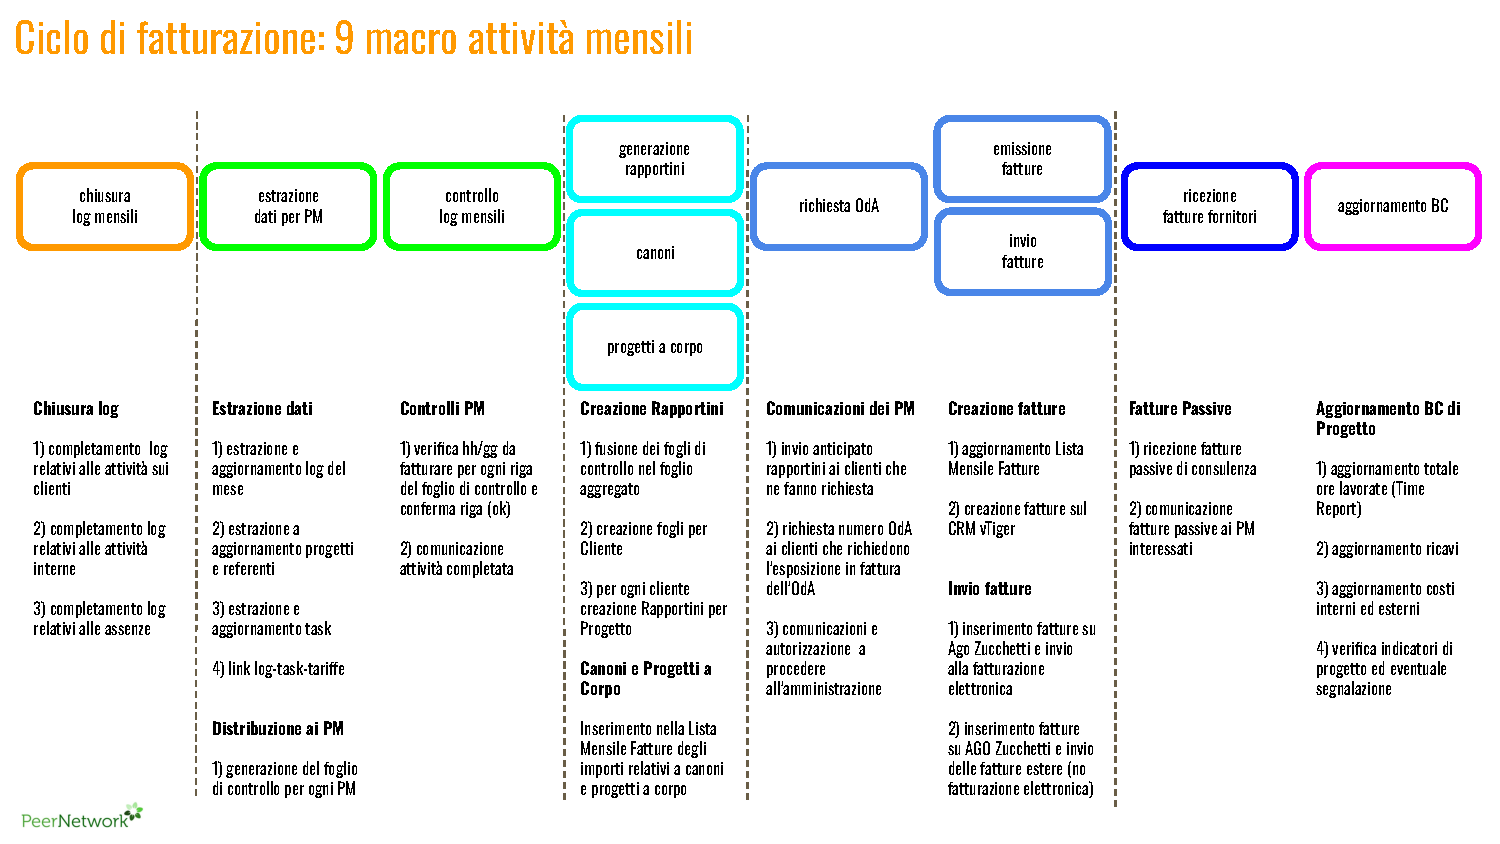
\includegraphics[width=\linewidth]{figures/fasiFatturazionePN.pdf}
    \caption{Attività presenti nel processo di fatturazione di \textit{Peer Network}}
    \label{fig:fatturazione}
\end{figure}

Le nuove funzionalità in fase di sviluppo, approfondite nel Capitolo \ref{chap:Results}, riguardano l’area dell’applicativo \ac{PAM} denominata \textbf{Progetti}, che verrà
utilizzata dalla direzione, dall’amministrazione e dai project manager. Questa sezione è pensata per centralizzare il controllo dei progetti, rendendo disponibili
informazioni generali, composizione dei team, tariffe orarie applicabili in base ai ruoli, situazione economica complessiva e dettagliata per mese, oltre alla
possibilità di consultare tutte le prefatture emesse.

Queste funzionalità semplificheranno notevolmente il lavoro degli utilizzatori, offrendo un unico punto di accesso per monitorare tutte le informazioni e mantenere
sotto controllo l’andamento dei progetti. Inoltre, la nuova gestione economica, sia generale che dettagliata, eliminerà la necessità di utilizzare i fogli elettronici
attualmente impiegati. Al momento, per ogni progetto viene creato un file separato per ogni anno solare, che deve essere aggiornato manualmente (come ultima fase del
processo di fatturazione nella \Cref{fig:fatturazione}) con i dati relativi a costi e ricavi effettivi, ricavi previsti per i mesi successivi e margini. Con la nuova area
Progetti, queste operazioni saranno automatizzate e integrate direttamente nell’applicativo.

\chapter{Strumenti e Tecnologie}
In questo capitolo vengono esaminati i principali strumenti e le tecnologie utilizzati durante lo svolgimento di tutte le attività, suddivisi in categorie
in base alla loro tipologia. Verranno trattati, con un approfondimento sul loro utilizzo pratico, gli ambienti di sviluppo integrati (IDE), i sistemi di
versionamento, i framework, le librerie e i linguaggi di programmazione, nonché le piattaforme per la gestione dei progetti e la collaborazione.
La scelta di queste tecnologie è stata influenzata principalmente dalle soluzioni già adottate da \textit{Peer Network} per la gestione e lo sviluppo dei progetti, 
oltre ad alcune proposte mirate a soddisfare esigenze operative specifiche.

\section{Strumenti}
\begin{itemize}
    \item \textbf{Jira}: strumento di gestione progetti e monitoraggio sviluppato da Atlassian, principalmente per i team di sviluppo software. Questo strumento
    supporta metodologie Agile e consente di creare, assegnare e monitorare le attività. Tutte le attività svolte sono state registrate, organizzate e monitorate
    in un apposito progetto. Ogni progetto è strutturato con una gerarchia di epic, task e subtask, permettendo di suddividere il lavoro in unità più piccole e
    gestibili, in modo da mantenere un controllo chiaro e dettagliato sui progressi. Gli elementi della gerarchia sono stati costantemente aggiornati con dettagli
    e stato corrente, garantendo una visione sempre aggiornata. Le ore di lavoro dedicate a ciascun task e subtask sono state registrate tramite una funzionalità
    specifica e monitorate facilmente con l’applicazione integrata \textbf{Time Tracker Lite}, utilizzando filtri per l’analisi dei dati. Per pianificare le varie attività
    da svolgere, è stata utilizzata la dashboard \textbf{Timeline}, che permette di avere una panoramica chiara delle scadenze e delle priorità. Jira è stato integrato con
    Confluence per collegare attività e documentazione dello stesso progetto.
    \item \textbf{Confluence}\footnote{\url{https://www.atlassian.com/software/confluence}}: strumento di collaborazione e gestione della conoscenza sviluppato da Atlassian, progettato per centralizzare la creazione, l'organizzazione
    e la condivisione di documenti e pagine. È stato utilizzato per documentare i progetti, raccogliere appunti e facilitare la collaborazione in tempo reale tra i colleghi.
    Integrato con Jira, ha permesso di collegare facilmente la documentazione alle attività monitorate, mantenendo coerenza tra sviluppo e gestione operativa. Ogni progetto
    è organizzato in uno spazio dedicato, dove sono raccolti resoconti di riunioni, documentazione tecnica e materiali di supporto, garantendo un accesso rapido e
    strutturato alle informazioni. La \textit{Peer Network} utilizza questo strumento per creare e mantenere una knowledge base aziendale, utile come riferimento per risolvere
    problemi ricorrenti e condividere best practice. Grazie alla sua flessibilità, Confluence ha reso possibile aggiornare costantemente i contenuti e organizzare le
    informazioni in modo chiaro e accessibile a tutti i dipendenti.
    \item \textbf{Bitbucket}\footnote{\url{https://bitbucket.org/}}: piattaforma di gestione del codice sorgente sviluppata da Atlassian, è stata utilizzata per tracciare e gestire in modo efficiente le
    modifiche al codice tramite il controllo di versione \textbf{Git}\footnote{\url{https://git-scm.com}}. L'azienda ha repository dedicati per ogni progetto, implementando rigorosi controlli di accesso che
    garantiscono sia la sicurezza che una gestione centralizzata del codice. Questa piattaforma aiuta la collaborazione tra i membri del team di sviluppo, consentendo
    a ciascun sviluppatore di contribuire al codice sorgente e monitorare in tempo reale le modifiche apportate dai colleghi.
    \item \textbf{Slack}\footnote{\url{https://slack.com/intl/it-it/}}: piattaforma di comunicazione e collaborazione aziendale progettata per ottimizzare il lavoro. Permette di inviare messaggi istantanei, effettuare
    chiamate vocali e video e condividere file in tempo reale. L’ambiente di lavoro \textit{Peer Network} è organizzato in canali tematici, suddivisi per progetto, reparto o argomento,
    facilitando la gestione delle conversazioni. Grazie all’integrazione con strumenti come Jira e Confluence, Slack supporta un flusso di lavoro collaborativo ed efficiente.
    Tutte le comunicazioni interne, sia tra colleghi che con l’azienda, sono state gestite tramite questa piattaforma, garantendo ordine e accessibilità alle informazioni.
    \item \textbf{Google Workspace}\footnote{\url{https://workspace.google.com/intl/it/}}: \textit{Peer Network} adotta un dominio aziendale dedicato tramite Google, fornendo a ciascun dipendente un account personalizzato
    per accedere agli strumenti e alle risorse condivise. Il \textbf{Google Drive} aziendale è stato utilizzato per archiviare, consultare e modificare file e cartelle, con permessi
    di accesso configurati per garantire sicurezza e controllo. I \textbf{Google Calendar} personali sono stati condivisi tra i dipendenti, facilitando la pianificazione di riunioni
    e attività. Le riunioni sono state programmate su Calendar e svolte in modalità mista, consentendo ai dipendenti in smart working di partecipare tramite \textbf{Google Meet}.
    Per le presentazioni, sono stati utilizzati \textbf{Google Slides}, sia per le riunioni interne che per quelle con i clienti. \textbf{Gmail} ha centralizzato tutte le notifiche aziendali,
    incluse quelle provenienti da strumenti come Jira, Confluence, Bitbucket e Slack, offrendo un unico punto di accesso per il monitoraggio delle comunicazioni e delle attività.
    \item \textbf{Miro}\footnote{\url{https://miro.com/it/}}: piattaforma di collaborazione online che ha semplificato la creazione e la condivisione in tempo reale di schemi e diagrammi, come la \textbf{\ac{WBS}},
    attraverso una lavagna virtuale accessibile a più colleghi simultaneamente. Miro è stato proposto all'azienda per sostituire l’uso di Google Slides, precedentemente impiegato
    per realizzare questi schemi senza uno strumento dedicato.
    \item \textbf{Visual Studio Code}\footnote{\url{https://code.visualstudio.com}}: editor di codice sorgente usato come IDE durante lo sviluppo. Grazie all'integrazione con Git e all'uso di alcuni plugin, ha consentito
    di gestire facilmente le operazioni di controllo versione direttamente dall’interfaccia grafica, semplificando il controllo del codice sorgente.
    \item \textbf{MySQL Workbench}\footnote{\url{https://www.mysql.com/products/workbench/}}: software dedicato alla gestione di database MySQL. Grazie alla sua interfaccia, è stato possibile consultare e interrogare il database di \ac{PAM}
    tramite la creazione e l’esecuzione di query SQL.
\end{itemize}

\section{Tecnologie}
\begin{itemize}
    \item \textbf{Vue.js}\footnote{\url{https://vuejs.org}}: framework JavaScript open-source progettato per la creazione di interfacce utente e applicazioni single-page. È noto per la sua reattività e
    facilità di integrazione con altre librerie. Basato su un’architettura a componenti, permette di organizzare il codice in moduli riutilizzabili e facilmente
    gestibili. Grazie ai suoi meccanismi reattivi, il \ac{DOM} si aggiorna automaticamente al variare dei dati, supportando direttive dinamiche
    per la manipolazione del contenuto. Questo strumento è stato impiegato per lo sviluppo frontend di \ac{PAM}.
    \item \textbf{Vuex}\footnote{\url{https://vuex.vuejs.org}}: libreria di gestione dello stato per Vue.js, progettata per centralizzare e organizzare i dati in un unico store. Facilita la gestione di
    applicazioni complesse grazie a un flusso strutturato di mutazioni, che consente di modificare lo stato in modo tracciabile e prevedibile. È particolarmente utile
    per condividere dati tra componenti senza la necessità di passaggi manuali. Questa libreria è stata utilizzata per lo sviluppo frontend di \ac{PAM}.
    \item \textbf{Liferay}\footnote{\url{https://www.liferay.com/it/}}: piattaforma open-source progettata per la creazione di portali web e siti aziendali, offrendo soluzioni personalizzate per la gestione di
    contenuti, applicazioni e servizi online. La sua architettura modulare garantisce elevata personalizzazione e scalabilità, rendendola adatta a progetti complessi.
    Supporta diversi framework e tecnologie, tra cui JavaScript, favorendo l’integrazione con strumenti moderni di sviluppo. Questa piattaforma è stata utilizzata per
    gestire il frontend di \ac{PAM}, ospitando il codice sviluppato in Vue.js.
    \item \textbf{JavaScript}\footnote{\url{https://developer.mozilla.org/en-US/docs/Web/JavaScript}}: linguaggio di programmazione utilizzato principalmente per lo sviluppo web. È eseguito direttamente nel browser e permette di creare
    pagine dinamiche e interattive. Viene utilizzato in Vue.js per creare e gestire i componenti e la logica dell'applicazione, oltre alla modifica dinamica del
    \ac{DOM} tramite direttive specifiche. Anche la gestione dello stato in Vuex è fatta in JavaScript.
    \item \textbf{MySQL}\footnote{\url{https://www.mysql.com/it/}}: sistema di gestione di database relazionali (RDBMS) utilizzato in \ac{PAM} per archiviare, organizzare e recuperare dati in modo strutturato.
    È stato possibile interagire con i dati tramite il linguaggio Structured Query Language (SQL). 
\end{itemize}

\chapter{Gestione Progetti}
\label{chap:pm}

Come già anticipato, questo capitolo approfondisce tutte le attività che costituiscono il ciclo di vita
di un progetto di \textit{Peer Network}, dalla fase di ideazione fino al rilascio al cliente e al supporto post-installazione.
L’analisi condotta ha permesso di individuare criticità lungo il processo e di elaborare proposte mirate alla loro risoluzione.

Nel corso del lavoro, è stato possibile seguire sia progetti già in corso che nuovi, partendo dalle riunioni
preliminari con i committenti per valutare l’opportunità di sviluppare un nuovo applicativo. Partecipare a incontri
con i clienti e con i team di progetto ha offerto una visione completa della gestione operativa e del lavoro
svolto dai diversi dipendenti, in particolare dai responsabili di progetto. Questa esperienza, oltre alla
consultazione di fonti di riferimento nel settore e all’esperienza maturata in altri contesti lavorativi,
ha permesso di sviluppare proposte concrete per migliorare i processi, adattandole alle reali esigenze dei
team senza stravolgerne il metodo di lavoro.

L'analisi e le proposte sviluppate si basano costantemente sulla struttura del ciclo di vita del progetto proposta dall'azienda
e illustrata nella Sezione \ref{sec:pm}.

\section{Analisi Stato}
I progetti per clienti esterni possono variare notevolmente in natura e, di conseguenza, nella durata che intercorre tra l’inizio e l'installazione:
\begin{itemize}
    \item aggiunta di funzionalità a un sistema esistente: da una a più settimane, a seconda della complessità;
    \item creazione di un nuovo applicativo con la maggior parte delle \ac{PBC} già presenti: da uno a diversi mesi;
    \item migrazione di un \ac{ERP} aziendale (ad esempio, da SAP ECC a SAP S/4HANA), oppure creazione di un nuovo
    applicativo con numerose \ac{PBC} da sviluppare e/o logiche nuove: oltre tre mesi. I progetti di grandi dimensioni
    vengono suddivisi in sotto progetti, ciascuno della durata massima di tre o quattro mesi, per consentire rilasci graduali stabilendo le priorità.
\end{itemize}

Le proposte per un progetto possono provenire da diverse fonti. Nel caso di un nuovo cliente, il CEO di \textit{Peer Network} verrà contattato direttamente.
Se il committente ha già progetti o collaborazioni attive con l’azienda, la proposta può essere inviata via posta elettronica o telefonicamente:
\begin{itemize}
    \item contattando il CEO;
    \item rivolgendosi al project manager di riferimento di un progetto in corso per la stessa azienda;
    \item contattando i responsabili del servizio di supporto. Questo è particolarmente utile quando inizialmente 
    il cliente ritiene di aver bisogno solo di una piccola miglioria in un'applicazione, ma dall'analisi della
    richiesta emerge la possibilità di sviluppare un nuovo progetto.
\end{itemize}

Un'ulteriore possibilità riguarda i progetti interni, nei quali non esiste un committente esterno, ma è la \textit{Peer Network} a essere cliente di sé stessa.

Nel caso di clienti esterni, tutte le richieste vengono sempre inoltrate al CEO, il quale gestisce l'intera fase iniziale del progetto.

    \subsection{Idea, Design, Economics}
    Sulla base di indicazioni formali e informali ricevute dai clienti, sia verbalmente che tramite email, il
    CEO elabora dei \textbf{mockup} utilizzando il software Axure\footnote{\url{https://www.axure.com}}. Se le funzionalità richieste sono già presenti in altre
    \ac{SBS}, verranno presentate schermate simili a quelle utilizzate da altri clienti. In caso contrario,
    si esamineranno soluzioni personalizzate per soddisfare le esigenze specifiche.

    Dopo alcune \textbf{riunioni con i clienti}, si definiscono in modo più o meno dettagliato i \textbf{requisiti} richiesti. Questi ultimi,
    tuttavia, non vengono quasi mai redatti in modo collaborativo. Se la soluzione proposta al cliente è già stata
    implementata per altri, non si parte da zero nella raccolta dei requisiti. In base alle richieste ricevute, il CEO
    valuta quali \ac{PBC} possono essere utilizzate; nel caso in cui non siano disponibili, informa gli sviluppatori e avvia
    immediatamente il processo di creazione.

    Successivamente, il cliente comunica la disponibilità delle sue \textbf{risorse}, ovvero le macchine virtuali su cui \textit{Peer Network}
    installerà gli ambienti di sviluppo, test e produzione. Inoltre, egli indica la data entro la quale desidera ricevere il sistema completo
    ed eventuali periodi in cui non sarà possibile lavorare per necessità aziendali.

    Una volta definiti i requisiti e le tempistiche per il completamento del progetto, il CEO redige un’\textbf{offerta} che il cliente
    accetta. Dopo aver preso in carico il progetto, egli crea uno spazio dedicato su Confluence per i \textbf{documenti interni}, dove
    inserisce un riassunto di quanto concordato. Ogni azienda cliente dispone
    di un proprio spazio Confluence personalizzato e condiviso, contenente tutta la documentazione rilevante per i suoi progetti.
    In questa fase iniziale, il CEO si occupa di aggiornare lo spazio con il nuovo progetto.

    Il \textbf{Project Management Life Cycle} adottato si basa su un approccio Agile, combinato con un modello iterativo personalizzato
    ispirato a Kanban. Lo scopo del progetto è definito fin dall'inizio e rimane invariato. Le soluzioni vengono sviluppate in
    piccoli passi: le attività sono organizzate in base alla priorità per garantire il rilascio progressivo e frequente di moduli,
    cioè parti applicative funzionanti coerenti tra loro e autoconclusive. Al termine dello sviluppo e del testing di ciascun modulo,
    questo viene rilasciato al cliente secondo le scadenze concordate. Idealmente, le persone responsabili indicate dal committente o
    gli utilizzatori del sistema dovrebbero eseguire test funzionali
    parallelamente al rilascio nell’ambiente di test, per verificare che i requisiti siano soddisfatti. Tuttavia, in molti casi, essi
    preferisco fornire feedback solo al completamento dell'intero lavoro.

    Il CEO è responsabile di questa fase, ricoprendo i ruoli di commerciale, analista e progettista. È lui a concordare con il cliente i requisiti, i costi e i tempi di realizzazione.

    Deliverables prodotti: mockup, documento richieste cliente (opzionale), offerta fatta al cliente.

    Ruoli interni coinvolti: CEO.

    Problemi riscontrati:
    \begin{itemize}
        \item mancano i verbali delle riunioni tenute con i clienti;
        \item non ci sono figure specifiche coinvolte, poiché le interazioni sono solo gestite dal CEO;
        \item frequentemente non viene stilato un elenco generico delle richieste, né tantomeno un insieme dettagliato
        di requisiti funzionali e non funzionali. Di conseguenza, nelle fasi successive ci si basa solo sui mockup e
        su informazioni riportate oralmente dal CEO;
        \item spesso non ci sono accordi definitivi con il cliente, il che porta a iniziare la fase successiva senza indicazioni
        chiare su budget e tempistiche. Questo comporta il rischio di dover effettuare un investimento interno;
        \item si utilizzano risorse umane sottratte dal lavoro operativo di sviluppo in altri progetti solo per chiedere consigli,
        fare ricerca di soluzioni simili già presenti presso i clienti e verificare le funzionalità nelle \ac{PBC} già sviluppate;
        \item spesso, i tempi e le scadenze stabilite con il cliente non sono sostenibili, dato l'alto numero di progetti in
        corso simultaneamente all'interno dell'azienda. Ciò aumenta il rischio di ritardi nelle consegne. Per evitare tali ritardi,
        tuttavia, si è costretti a ridurre significativamente la qualità del codice, della documentazione di gestione del progetto e tecnica,
        che risultano quasi assenti;
        \item non sono stati stabiliti deliverables standard da produrre in questa fase.
    \end{itemize}

    \subsection{Progetto Software}
    Per \textit{Peer Network}, il project manager entra in gioco in questa fase, assumendo un ruolo cruciale nella riuscita del progetto.
    Questa figura professionale è responsabile della gestione ottimale delle risorse assegnate, del monitoraggio delle attività
    e del rispetto dei tempi e delle scadenze. Inoltre, egli coordina il team di progetto, che include sia risorse interne all'azienda
    sia quelle del cliente. Egli dovrebbe aggiornare costantemente su Confluence sia lo spazio del cliente che quello interno all'azienda,
    inserendo tutti i documenti che ritiene necessari.

        \subsubsection{Avvio}
        Il project manager avvia il processo di gestione del progetto analizzando le richieste ricevute dal CEO. Questo include la
        revisione dei mockup o presentazioni su Google Slides, insieme ad un eventuale documento riepilogativo delle esigenze del cliente.

        Successivamente, il project manager e il CEO organizzano una \textbf{piccola riunione} per presentare il nuovo progetto a un gruppo
        ristretto di persone potenzialmente coinvolte nel team. Questo incontro è raramente condotto in presenza dei clienti. A parte
        il project manager, gli altri membri del gruppo hanno solo una comprensione generale delle aree di intervento, senza che venga designato un team leader o altri ruoli ufficiali.
        
        Il project manager è responsabile del \textbf{business case} del progetto, un foglio elettronico in cui viene inserita l'analisi dei \underline{costi}
        e dei \underline{ricavi pianificati}. Considerando il budget e i tempi concordati con il cliente nella fase iniziale, il compito del project manager
        è quello di trovare il modo migliore per rimanere all'interno di questi limiti. A tal fine, egli stima il numero di giorni/persona necessari
        per completare il lavoro e, utilizzando il costo orario di un dipendente, calcola il costo totale interno pianificato. Partendo da queste
        informazioni e dal budget, si può determinare quanto ricavo e margine sono pianificabili.

        Deliverables prodotti: business case.

        Ruoli interni coinvolti: project manager, CEO.

        Problemi riscontrati:
        \begin{itemize}
            \item non esiste un metodo standard per affrontare questa fase, quindi ogni project manager la affronta a propria discrezione;
            \item la documentazione di progetto relativa a questa fase, in particolare quella riguardo ai requisiti, viene redatta solo sporadicamente.
            Di conseguenza, nelle fasi successive il project manager è sempre costretto a rivolgersi al CEO per ottenere chiarimenti, anche da parte degli sviluppatori;
            \item spesso, non c’è un team di progetto definito, poiché si coinvolgono gli sviluppatori disponibili o adatti ai compiti richiesti in base alle esigenze del momento;
            \item i ruoli all'interno del gruppo non vengono quasi mai assegnati in modo formale;            
            \item non sono stati stabiliti deliverables standard da produrre in questa fase.
        \end{itemize}

        \subsubsection{Pianificazione}
        Partendo dall’idea e dalle funzionalità, a volte il project manager sviluppa una \textbf{\ac{WBS}}, scomponendo il progetto in
        numerosi elementi organizzati in una gerarchia chiara, simile a un diagramma ad albero. Dallo schema devono emergere chiaramente le
        funzionalità specifiche da sviluppare e i moduli in cui si intende dividere il progetto. Un modulo è definito come un insieme di funzionalità
        coerenti, che possono essere rilasciate in modo indipendente dalle altre, garantendo che ciascun modulo sia autoconclusivo. Idealmente, ogni
        volta che viene rilasciato un modulo, il cliente ha la possibilità di testarne le funzionalità. È fondamentale che la \ac{WBS} sia comprensibile
        anche per il cliente, pertanto, viene presentata a un livello logico non tecnico, mantenendo comunque il giusto grado di dettaglio.
        Nella Figura \ref{fig:wbs-esismart} è rappresentato un estratto della \ac{WBS} del progetto reale “esiSMART2”, elaborata dal project manager responsabile e
        presentata al cliente l'anno scorso. La radice rappresenta il modulo di riferimento, mentre gli altri elementi indicano le diverse
        funzionalità richieste, con un livello di dettaglio sempre crescente.

        \begin{figure}
            \centering
            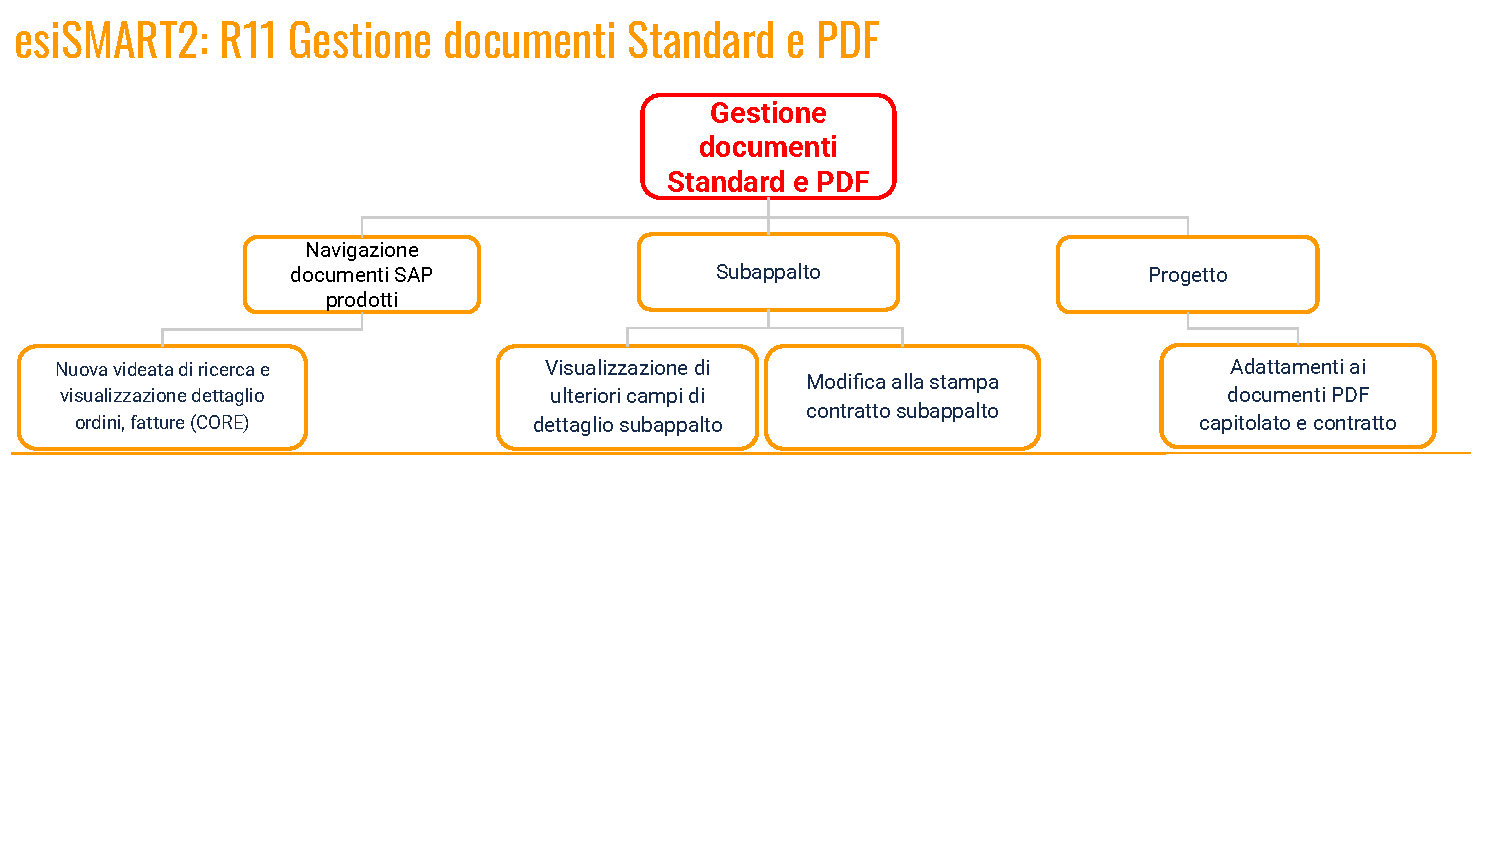
\includegraphics[width=\linewidth]{figures/esismartWBS.pdf}
            \caption{Parte di una WBS per un progetto cliente, modulo “Gestione documenti Standard e PDF”}
            \label{fig:wbs-esismart}
        \end{figure}

        È successo raramente che si effettuasse un'\textbf{analisi dei rischi}, la quale veniva condotta dopo aver scomposto il problema in moduli
        e relative funzionalità. Questo approccio è stato adottato in progetti in cui si prevedevano significative criticità in alcuni moduli.
        A seguito dell'analisi, si valutava come mitigare o risolvere il problema, riportando le informazioni al cliente e condividendo una possibile strategia.

        Per avere una visione complessiva del progetto, il project manager elabora un \textbf{Gantt}, posizionando tutti i moduli da sviluppare all'interno di un
        calendario. Questo processo tiene conto delle scadenze concordate con il cliente e delle dipendenze tra i vari moduli. Non tutti i project manager
        seguono questa prassi; coloro che lo fanno, utilizzano lo strumento GanttPro\footnote{\url{https://ganttpro.com/it/}}. Talvolta, prima di redigere il Gantt, si crea uno \textbf{schema generale di pianificazione
        rilasci} fino al lancio, privo di date, ma che evidenzia l’ordine dei rilasci (come illustrato nella Figura \ref{fig:schema-rilasci}). In entrambi i casi, la pianificazione
        viene sottoposta a validazione da parte del cliente.

        \begin{figure}
            \centering
            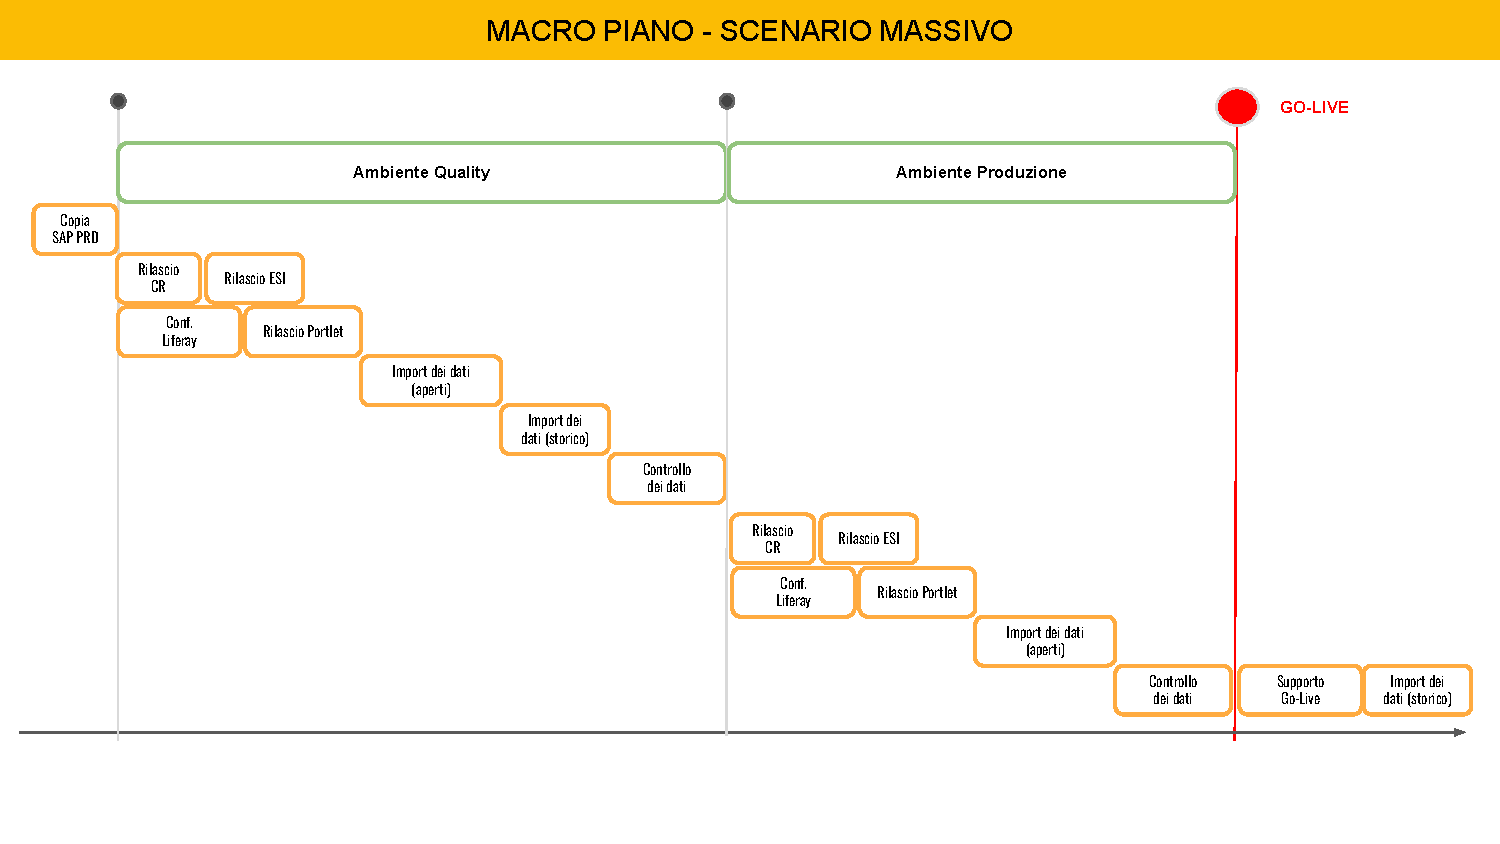
\includegraphics[width=\linewidth]{figures/pianoRilasci.pdf}
            \caption{Schema generale di pianificazione dei rilasci}
            \label{fig:schema-rilasci}
        \end{figure}

        Per ogni progetto, il project manager, o il CEO, crea un \textbf{progetto su Jira}, inserendo le informazioni nella dashboard Timeline:
        \begin{itemize}
            \item Partendo dalla \ac{WBS}, i moduli identificati in precedenza vengono inseriti come \underline{epic}. Questi rappresentano
            delle milestone di progetto e vengono rilasciati al loro completamento. A causa del suo livello logico generale, una epic non può essere
            assegnata a una persona specifica, il che significa che nessuno sviluppatore può indicare direttamente il tempo impiegato per il suo sviluppo. Ad
            esempio, come illustrato nella Figura \ref{fig:wbs-esismart}, una epic potrebbe essere “R11 Gestione documenti Standard e PDF“, dove R11 indica che sarà l’undicesimo modulo da rilasciare.

            \item Ogni epic è ulteriormente scomposta in:
                \begin{itemize}
                    \item \underline{user stories} (opzionale): rappresentano la descrizione di una funzionalità e sono formulate in una semplice frase seguendo
                    il modello standard ruolo-goal-beneficio del framework Agile Scrum. A causa del loro livello di generalità, non possono essere
                    assegnate a una persona specifica, rendendo impossibile per gli sviluppatori indicare il tempo necessario per il loro sviluppo. Le
                    user stories non sono sempre presenti, poiché la loro necessità dipende dalla natura del progetto e, se ritenute utili, vengono
                    redatte durante l’analisi funzionale e assegnate alle rispettive epic. Nel caso siano presenti, da queste si derivano i task, ovvero le
                    attività necessarie per soddisfare le richieste.

                    \item \underline{task}: sono le attività da svolgere che, pur essendo di un livello non tecnico, rappresentano l'ultimo tipo di elemento
                    comprensibile per il cliente. Essi facilitano anche la comunicazione con il committente e hanno già un carattere operativo. Ogni task
                    viene assegnato a una persona responsabile del suo sviluppo e la gestione di queste attività è compito del project manager. Ogni
                    dipendente al quale viene assegnato un task può caricare il tempo impiegato per lavorare a questa attività. Ad esempio, come mostrato
                    nella Figura \ref{fig:wbs-esismart}, per ogni foglia dello schema viene creato un task con un titolo descrittivo, che fa riferimento anche al nodo padre.
                \end{itemize}
            
            \item Ogni task è suddiviso in \underline{subtask}, che rappresentano attività tecniche non rilevanti per il cliente, poiché si trovano a un livello
            implementativo. Anche questi compiti vengono assegnati a una persona responsabile dello sviluppo. Idealmente, dovrebbe occuparsene il team leader, ovvero il
            responsabile incaricato degli aspetti tecnici. Tuttavia, in molte occasioni, non viene nemmeno
            nominato e quindi anche questo compito ricade sul project manager. I dipendenti possono caricare le ore di lavoro su ogni subtask.
        \end{itemize}

        Per ogni elemento inserito nel progetto Jira è buona prassi fornire descrizioni testuali, immagini e link a documenti pertinenti
        (sul progetto Confluence associato), così da garantire spiegazioni più dettagliate.
        Molto spesso, non tutte le epic e i task vengono scomposti inizialmente rispettivamente in task e subtask, così da seguire un approccio iterativo.
        Questo implica che i primi elementi da sviluppare verranno raffinati con la maggiore granularità possibile fin da subito. Gli altri, invece,
        saranno analizzati progressivamente durante il progetto.
        Nella Figura \ref{fig:timeline-jira-progetto} è mostrato un esempio di progetto su Jira. Nella Timeline, le epic sono rappresentate da icone viola. Ogni epic include task
        contrassegnati da un'icona azzurra con una spunta. Nella finestra a destra, è visibile il dettaglio del task, completo di spiegazioni e immagini,
        insieme ai subtask, che sono indicati come “child issues” e un'icona azzurra.
        
        \begin{figure}
            \centering
            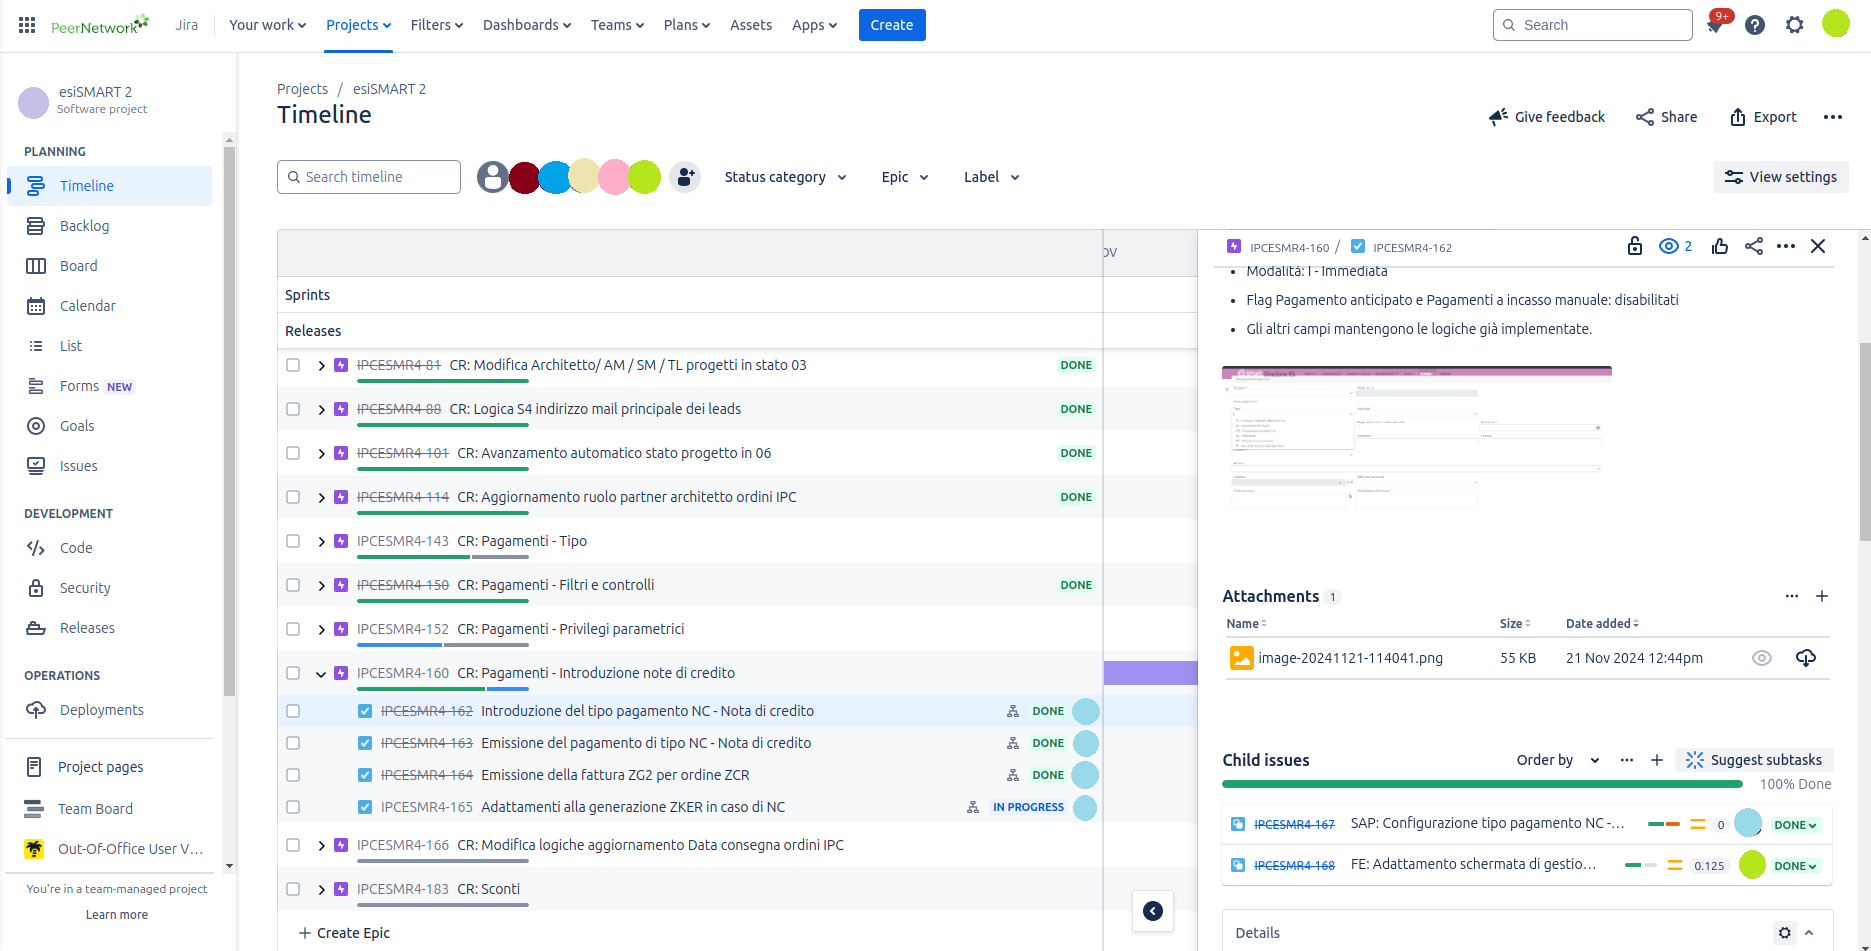
\includegraphics[width=\linewidth]{figures/timelineJira.png}
            \caption{Timeline di un progetto su Jira}
            \label{fig:timeline-jira-progetto}
        \end{figure}

        Per quanto riguarda le \textbf{risorse umane} assegnate a task e subtask, è importante notare che, man mano che le attività si allontanano nel tempo,
        aumenta l'incertezza riguardo alle persone specifiche che si occuperanno di esse. Tuttavia, per una prima suddivisione, si assegnano risorse
        generiche, come ad esempio frontend developer, ABAP\footnote{ABAP è un linguaggio di programmazione creato e utilizzato da SAP.} developer o backend developer.
        
        Una volta completata la suddivisione, si passa alla \textbf{pianificazione} nella Team Board di Jira, organizzando le attività a lungo termine.
        In questa fase, si stabilisce l'ordine di sviluppo delle epic e dei task, insieme alla loro durata, seguendo lo schema Gantt definito inizialmente.
        A seconda delle dimensioni del progetto, si utilizzano i mesi o le settimane come unità di misura. Questa fase è cruciale per comprendere se nel lungo
        periodo ci sarà bisogno di dipendenti con competenze specifiche. Ad esempio, se tra due mesi saranno necessari cinque sviluppatori ABAP,
        è fondamentale verificare se ci sono risorse umane interne disponibili in quel periodo per occuparsi di questo progetto.
        In caso contrario, sarà necessario cercare e assumere nuovi dipendenti in tempo utile.

        Deliverables prodotti: \ac{WBS} (opzionale), Gantt (opzionale), schema di pianificazione rilasci (opzionale), analisi rischi (opzionale), pianificazione.

        Ruoli interni coinvolti: project manager, team leader (opzionale).

        Problemi riscontrati:
        \begin{itemize}
            \item non esiste un template standard della \ac{WBS};
            \item i project manager riscontrano difficoltà nel capire come scomporre e con quale granularità l’idea iniziale in una \ac{WBS} completa;
            \item la maggior parte delle volte, i project manager non fanno la \ac{WBS} e scompongono il problema direttamente sul relativo progetto Jira;
            \item non tutti i project manager utilizzano il diagramma di Gantt;
            \item nelle epic, user stories, task e subtask non sempre vengono fornite descrizioni o link a documenti pertinenti con spiegazioni più dettagliate;
            \item esiste una notevole confusione riguardo all'organizzazione di un progetto su Jira in epic, task e subtask e
            ogni project manager adotta un approccio diverso dagli altri;
            \item non c'è coerenza nella suddivisione dei task, il che porta a progetti privi di subtask o che ne contengono solo alcuni;
            \item non esiste un team di progetto ben definito, quindi una persona potrebbe avere task o subtask assegnati su tutti i progetti aziendali nella stessa settimana;
            \item poiché non ci sono team definiti, anche i ruoli non sono specificati, ad esempio, un project manager potrebbe trovarsi a svolgere attività di sviluppo in un altro progetto.
            Di conseguenza, le persone spesso faticano a comportarsi secondo il ruolo necessario in quel momento;
            \item i project manager, essendo anche figure tecniche, spesso non si concentrano su una pianificazione di livello logico
            dettagliata, ma tendono a passare direttamente allo sviluppo;
            \item la pianificazione risulta complessa, poiché l’approccio dei project manager tecnici è quello di non fornire stime su aspetti incerti, come la previsione
            dei tempi per attività future;
            \item i subtask sono frequentemente gestiti dal project manager, sia per l'assenza di un team leader sia perché non vuole
            delegare e si occupa direttamente delle attività;
            \item non sono stati stabiliti deliverables standard da produrre in questa fase.
        \end{itemize}

        \subsubsection{Esecuzione}
        La \textbf{programmazione} è l’organizzazione delle attività su un orizzonte temporale breve. Questa viene fatta settimanalmente dal project manager assegnando
        task e subtask raffinati ai dipendenti specifici. Ogni venerdì, il responsabile tecnico dell’azienda controlla che nella settimana successiva tutti gli
        sviluppatori siano occupati in attività e che tutti i task e subtask programmati per quel periodo siano assegnati a persone reali (quindi non siano più
        assegnati a risorse generiche). Nella Figura \ref{fig:programmazione-jira-progetto} c'è una visione dello schema Gantt del plugin Team Board su Jira, dove si vede la programmazione effettiva.
        Visto che ad ogni persona vengono assegnati più task e subtask da sviluppare, è suo compito registrare le ore di lavoro che impiega per ciascuno,
        oltre a spiegare quali attività ha svolto e aggiornarne lo stato di avanzamento (da completare, in corso, testato, completato).

        \begin{figure}
            \centering
            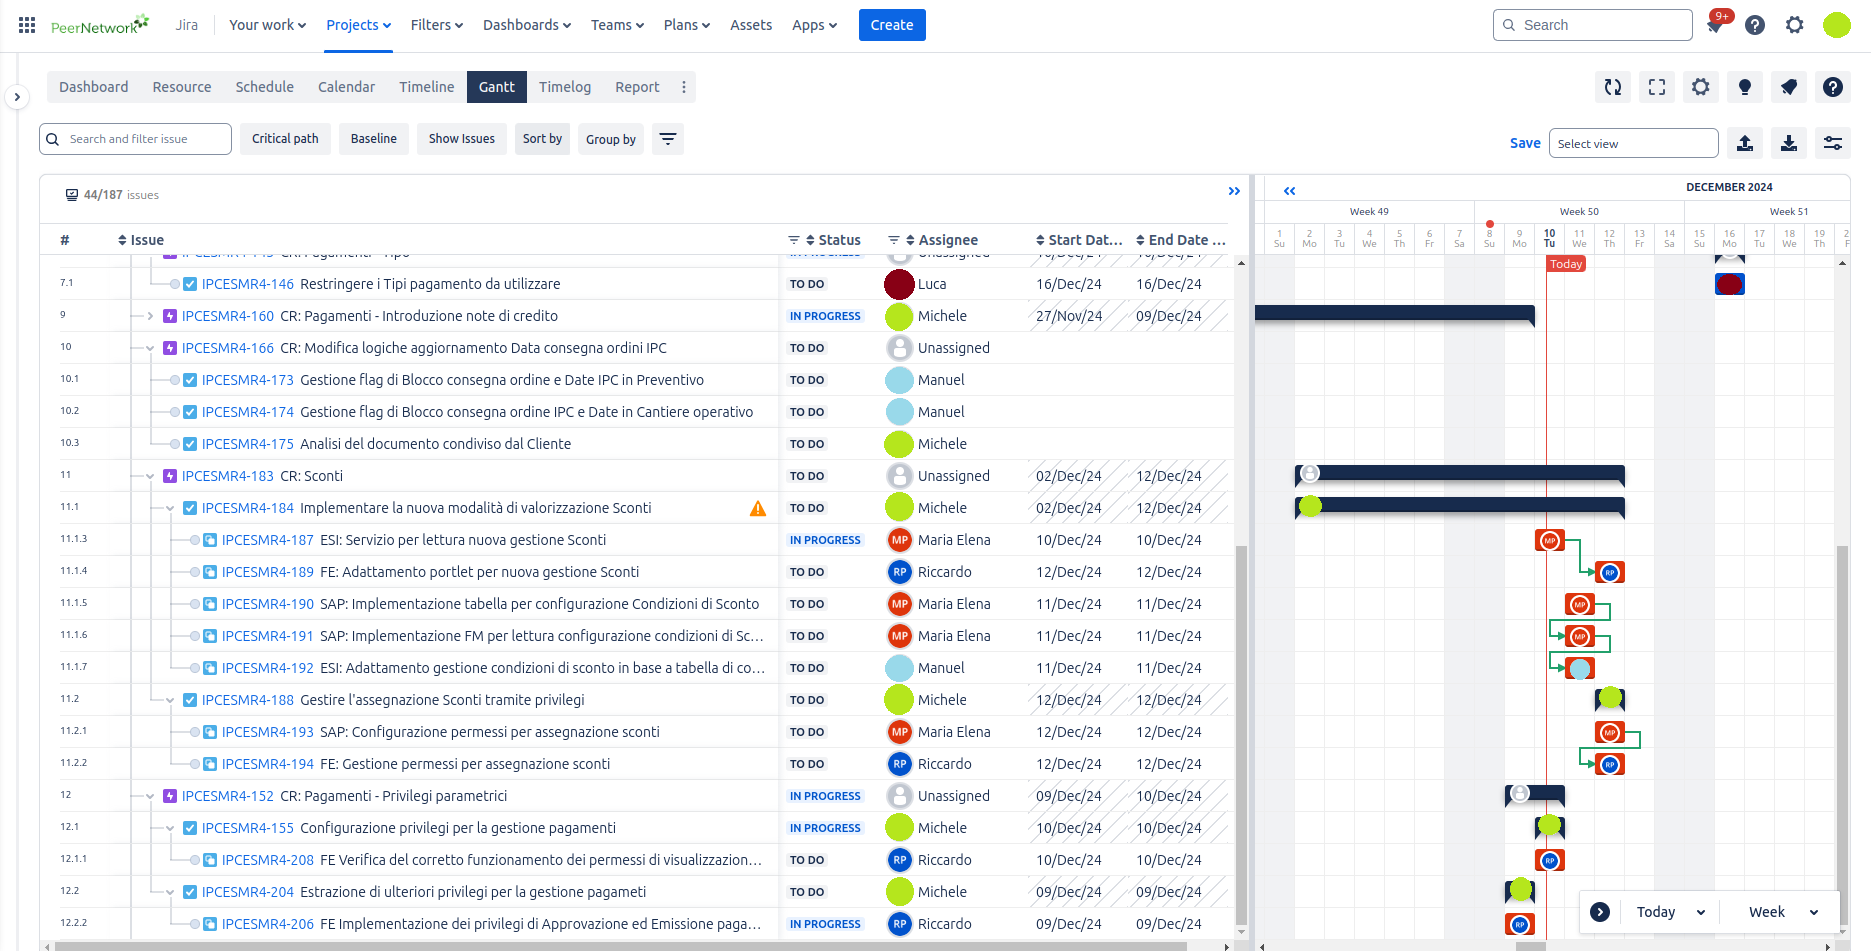
\includegraphics[width=\linewidth]{figures/programmazioneAttivita.png}
            \caption{Programmazione delle attività di un progetto}
            \label{fig:programmazione-jira-progetto}
        \end{figure}

        Durante lo \textbf{sviluppo}, i dipendenti caricano le modifiche al codice nel repository di progetto su Bitbucket, utilizzando le funzionalità del sistema
        di controllo di versione Git. Grazie all’integrazione tra gli strumenti Atlassian, è sufficiente adottare una convenzione standard per i nomi dei
        branch e dei commit affinché questi vengano associati automaticamente ai rispettivi task o subtask di Jira. Questo meccanismo permette di semplificare
        le attività di controllo e verifica. I commit devono seguire il formato \texttt{<codice Jira del task o subtask> <tipo di commit>: <descrizione>} (la
        seconda parte segue il Conventional Commit\footnote{\url{https://www.conventionalcommits.org/en/v1.0.0/}}), mentre per i branch si utilizza il formato \texttt{<codice Jira del task o subtask>-<descrizione>}.

        Il \textbf{rilascio del software} avviene esclusivamente in modo manuale, poiché non sono presenti meccanismi automatizzati come \textbf{continuous integration}
        o \textbf{continuous delivery}. Questa modalità dipende dall'attuale configurazione, in cui le repository di progetto risiedono su Bitbucket, una piattaforma
        in cloud, e l’accesso alle macchine virtuali dei clienti richiede l’utilizzo della VPN. Al momento, non sono state individuate soluzioni per superare le limitazioni
        legate all'accesso alle macchine virtuali tramite Bitbucket.

        Per quanto riguarda il \textbf{workflow di rilasci e test prima del rilascio in produzione}, il processo inizia nell'\underline{ambiente di sviluppo}, noto come DEV.
        Sebbene sia buona prassi eseguire gli Unit Test in questo ambiente, in realtà vengono svolti raramente a causa della mancanza dei dati necessari negli \ac{ERP},
        rendendo difficile condurre test significativi. Quando le funzionalità sono considerate stabili, si procede con il rilascio nell'\underline{ambiente di test} denominato
        QUALITY. In questa fase, è possibile rilasciare in modo indipendente componenti di frontend, \ac{ESI} o backend. Nel caso in cui non sia possibile eseguire Unit
        Test su DEV, questi vengono effettuati in QUALITY. In questo ambiente, gli sviluppatori eseguono anche Use Case
        Test e test funzionali, verificando manualmente che tutto funzioni correttamente in base alle user stories identificate in precedenza o alle richieste del cliente.
        Inoltre, in QUALITY i clienti dovrebbero eseguire gli User Acceptance Test man mano che le funzionalità vengono rilasciate, per assicurarsi che quanto sviluppato
        risponda alle loro esigenze. Qualora i committenti effettuino i loro controlli, possono inviare i riscontri tramite posta elettronica, telefonata o attraverso il service
        management di Jira. Tuttavia, non tutti i clienti sono disposti a testare progressivamente, poiché alcuni preferiscono che i cambiamenti vengano direttamente
        trasferiti in PROD, fornendo riscontri solo al termine del lavoro. Se tutto risulta stabile e accettato, i cambiamenti vengono trasferiti nell'ambiente di produzione,
        come descritto nella fase successiva. In alcuni casi, ci sono
        committenti che non dispongono di un ambiente di QUALITY, pertanto il rilascio avviene direttamente da DEV a PROD.

        In merito al \textbf{monitoraggio delle attività operative}, il project manager effettua una verifica settimanale dello stato di avanzamento del progetto utilizzando Jira.
        In alternativa, può consultare il team leader del progetto, se disponibile, o interagire direttamente con gli sviluppatori. Non è prevista una riunione fissa e gli
        aggiornamenti vengono forniti verbalmente. In presenza di \underline{problemi gravi}, il team leader, uno sviluppatore esperto o il project manager prepara un
        documento tecnico contenente una spiegazione dettagliata e le possibili soluzioni. Il project manager lo revisiona e lo adatta per renderlo comprensibile
        al cliente. Successivamente, il committente viene contattato telefonicamente o via email con il documento allegato e si organizza una videochiamata per
        presentare il problema e le soluzioni proposte dal team leader. Durante l'incontro, si concorda insieme al cliente la linea d'azione da seguire.
        Per \underline{problemi minori}, come uno sviluppatore che non comprende il task assegnatogli, non viene redatto un documento, ma si discute direttamente per
        risolvere la questione. Se si tratta di un problema tecnico, si coinvolge un esperto per ricevere assistenza. Nel caso di un \underline{problema} che può essere 
        \underline{interessante per tutti}, viene
        creato un documento su Confluence che spiega il problema e la relativa soluzione. Questo documento sarà accessibile a chiunque, così che possa essere utilizzato quando si presenterà un problema simile.
        In ogni caso, c'è sempre una collaborazione attiva tra tutti i dipendenti dell’azienda, in caso di necessità.

        All'inizio di progetti di grandi dimensioni, o in quelli che coinvolgono nuovi membri, si tiene al mattino uno \textbf{stand up meeting} informale di dieci minuti.
        Durante questa breve riunione, i partecipanti discutono i problemi emersi il giorno precedente e possono richiedere supporto per la giornata corrente. Alcuni
        progetti si prestano naturalmente a questo tipo di incontro, mentre altri potrebbero non essere adatti. La necessità di un stand up meeting dipende anche
        dalla dinamica del team: se i membri sono molto affiatati, esiste già un'intesa e un metodo di lavoro consolidato. Inoltre, la durata del progetto influisce
        sulla necessità di questa breve riunione, poiché per progetti di poche settimane, un incontro quotidiano potrebbe non essere necessario.

        Per un efficace \textbf{monitoraggio economico} del progetto, è fondamentale controllare sistematicamente il business case su base mensile.
        Questo implica un'analisi dei costi e dei ricavi pianificati, stabiliti all'inizio del progetto, confrontati con i \underline{costi e i ricavi effettivi}.
        I valori reali si aggiornano progressivamente, in base alle ore impiegate dai dipendenti nello sviluppo del progetto. 
        Il project manager ha il compito di monitorare costantemente questi valori, al fine di anticipare eventuali criticità, poiché il suo
        obiettivo è massimizzare il \underline{margine}. Se il progetto si estende all'anno solare successivo, ai project manager viene richiesto di elaborare una previsione
        dei costi e dei ricavi anche per quel periodo, così da avere un'idea chiara delle aspettative. 
        Ogni mese di sviluppo del progetto, i costi e i ricavi effettivi vengono aggiornati per quel periodo, mentre i costi e i ricavi pianificati per il mese successivo
        vengono rivisti in base ai dati effettivi del mese corrente, poiché questi ultimi sono considerati più affidabili.

        La frequenza degli \textbf{allineamenti con il cliente} è una scelta concordata ad inizio progetto e modificabile durante la sua esecuzione. Di solito,
        il project manager organizza incontri settimanali. Per progetti di minore entità, come piccole modifiche a sistemi esistenti, si decide
        settimanalmente con il cliente quali sviluppi intraprendere e rilasciare in quella settimana. Per progetti a lungo termine già ben pianificati, gli
        allineamenti avvengono almeno ogni due mesi. Alcuni project manager documentano sempre questi incontri e li pubblicano nello spazio Confluence del cliente.

        Il project manager è responsabile della pubblicazione di vari documenti nello spazio Confluence del committente, selezionando quelli che possono risultare
        utili in base alle esigenze specifiche del progetto. Tra i \textbf{documenti condivisi} possono figurare la documentazione tecnica richiesta, i problemi riscontrati e le soluzioni adottate.

        Deliverables prodotti: documentazione tecnica (su richiesta), documentazione codice, business case aggiornato, verbali allineamenti cliente (opzionale).

        Ruoli interni coinvolti: project manager, sviluppatori, team leader (opzionale).

        Problemi riscontrati:
        \begin{itemize}
            \item i project manager e i responsabili non hanno una visione chiara dello stato generale del progetto, poiché non tutti i dipendenti aggiornano in modo corretto e tempestivo
            lo stato di avanzamento dei task e subtask a loro assegnati;
            \item non tutti i dipendenti seguono le linee guida riguardo la nomenclatura di commit e branch;
            \item assenza di meccanismi per il rilascio e i test automatici;
            \item c'è una scarsa propensione alla documentazione su Confluence riguardo a quanto realizzato;            
            \item non tutti i project manager verbalizzano gli allineamenti con il cliente, perndendo così informazioni preziose;
            \item non è stata definita una lista di documenti importanti da pubblicare sistematicamente per ogni progetto nello spazio Confluence del cliente;
            \item non sono stati stabiliti deliverables standard da produrre in questa fase.
        \end{itemize}

        \subsubsection{Rilascio}
        La frequenza dei \textbf{rilasci in produzione} viene concordata con i clienti all'inizio del progetto, ma può essere modificata anche durante lo sviluppo.
        I tipi di rilascio standard sono i seguenti:
        \begin{itemize}
            \item settimanali: per moduli di piccole dimensioni;
            \item bisettimanali: per moduli che richiedono un'analisi aggiuntiva;
            \item mensili: per moduli che necessitano di una quantità significativa di test.
        \end{itemize}  
        
        In produzione è possibile rilasciare solo un modulo completo, comprendente di frontend, \ac{ESI} e backend correlati, affinché sia completamente funzionante.
        All'inizio di un nuovo progetto, il primo componente ad essere caricato in produzione è \ac{ESI} contenente le \ac{PBC} core, poiché comprendono
        tutte le funzionalità di utilità base necessarie per il corretto funzionamento generale del sistema.
        Il rilascio del software avviene esclusivamente in modo manuale, come descritto nella fase precedente.
        
        Generalmente, il \textbf{termine di un progetto} non è gestito in modo convenzionale, poiché non presenta una vera e propria conclusione. Infatti, c'è un continuo
        supporto e servizio di assistenza, come spiegato meglio nella fase successiva. Un progetto si considera concluso solo quando l'azienda cliente smette di utilizzare l'applicazione.
        Per quanto riguarda un progetto di migrazione, la conclusione del progetto è necessaria, in quanto coincide con il completamento del passaggio al nuovo sistema.
        In questo contesto di migrazione, viene organizzata una \textbf{retrospettiva
        interna} dedicata principalmente al team di progetto. La \textbf{retrospettiva con il cliente}, invece, viene effettuata solo su richiesta del committente stesso o quando è
        necessario affrontare aspetti critici, un’esigenza più comune nei progetti di grandi dimensioni.
        La retrospettiva è guidata dal project manager e condotta dal team leader insieme all’intero gruppo. Durante l’incontro, si analizzano e si confrontano le esperienze
        vissute durante il progetto, favorendo uno scambio di opinioni costruttivo.
        Nei progetti che comportano cambiamenti evolutivi su sistemi esistenti, non si prevedono retrospettive, poiché la loro durata è generalmente troppo breve per giustificare tale attività.
        
        Deliverables prodotti: soluzione prodotta, retrospettiva interna (opzionale), retrospettiva cliente (opzionale).

        Ruoli interni coinvolti: project manager, team leader (opzionale), sviluppatori.

        Problemi riscontrati:
        \begin{itemize}
            \item assenza di meccanismi automatici per il rilascio e i test;
            \item mancanza di un documento di rilascio finale;
            \item la riunione di retrospettiva viene fatta sporadicamente e solo per i progetti in cui ci sono stati aspetti negativi da segnalare;
            \item non sono stati stabiliti deliverables standard da produrre in questa fase.
        \end{itemize}

    \subsection{Supporto e Servizio}
    Dopo circa uno o due mesi dalla consegna ufficiale del sistema al cliente, quando è installato e considerato stabile, avviene il trasferimento della
    responsabilità del progetto al team di supporto. Per questo motivo, per ogni cliente viene creato un progetto su Jira per l'Application Management Service (AMS),
    così che il gruppo di supporto possa indicare in dettaglio tutte le attività svolte, nonché pianificarle e registrare le ore lavorate.

    I clienti possono comunicare con il team attraverso la segnalazione di problemi (noti come ticket) nel Jira Service Management, un ecosistema progettato per
    guidarli nella corretta formulazione delle richieste di supporto, manutenzione o evoluzione. In generale, per ogni segnalazione viene effettuata un'analisi
    del problema riportato e, in base alle richieste, vengono intraprese attività di correzione o sviluppo.

    Il team di supporto si occupa di diversi compiti, tra cui:
    \begin{itemize}
        \item \textbf{ricezione e classificazione delle segnalazioni}: un membro del team controlla quotidianamente ogni richiesta per verificare che il cliente abbia correttamente indicato gravità,
        priorità e tipologia di problema. Il team stima le ore o i giorni necessari per le attività da svolgere per ciascun ticket mentre analizza il problema riportato. Si identificano tre tipi di ticket: 
            \begin{itemize}
                \item malfunzionamento: viene riscontrato un piccolo problema nel sistema, quindi è necessaria una manutenzione correttiva;
                \item incident: il sistema non lavora correttamente e, di conseguenza, il cliente sta perdendo lavoro e denaro;
                \item cambiamenti: modifiche o aggiunta di funzionalità, cioè richieste evolutive.
            \end{itemize}
        \item \textbf{assistenza e supporto al cliente}: il team risponde a qualsiasi dubbio o richiesta del cliente, anche quando quest'ultimo non ricorda come eseguire una determinata operazione;
        \item \textbf{attività di manutenzione correttiva}: nel caso di malfunzionamenti o incident, normalmente le modifiche da fare sono relativamente piccole;
        \item \textbf{gestione delle richieste evolutive}: quando viene richiesto un cambiamento o l'aggiunta di funzionalità, se le attività necessarie hanno
        una durata stimata inferiore ai due giorni, il team di supporto se ne occupa direttamente. Altrimenti, la richiesta viene inoltrata ad un project manager di
        riferimento del progetto di sviluppo, il quale si occuperà di assegnare il lavoro agli sviluppatori. A seconda della complessità delle modifiche, il responsabile
        può decidere di organizzare un nuovo progetto con un team di sviluppo dedicato.        
    \end{itemize}

    Il team di supporto si occupa di integrare la \textbf{documentazione tecnica} relativa a ciascun progetto su Confluence, riportando tutte le modifiche apportate.
    Qualora alcune soluzioni siano state implementate in modo tale da risultare utili anche per altri progetti, queste vengono dettagliate in uno spazio di Confluence
    interno all’azienda, accessibile a tutti i dipendenti. Tuttavia, queste informazioni vengono raramente condivise con il cliente, poiché si tratta di aspetti
    tecnici che non sono di suo interesse. Inoltre, poiché in molti progetti la documentazione generale è carente, non è opportuno condividere la parte relativa alla
    manutenzione, in quanto risulta incompleta per definizione.

    Deliverables prodotti: documentazione interna del progetto aggiornata.

    Ruoli interni coinvolti: team di supporto.

    Problemi riscontrati:
    \begin{itemize}
        \item il team si trova in difficoltà nel comprendere dove e come intervenire, a causa di:
            \begin{itemize}
                \item la documentazione del codice (Javadoc) è quasi inesistente e il codice stesso è poco commentato (spiegazione di logiche complesse);
                \item la documentazione di progetto è caotica e insufficiente.
            \end{itemize}
        \item ci sono numerosi ritardi nelle consegne, poiché spesso si stima che la risoluzione di un task richieda poco tempo,
        ma poi si scopre codice poco manutenibile e debito tecnico, per colpa di:
            \begin{itemize}
                \item il sistema del cliente è obsoleto e non è stato aggiornato in concomitanza con le modifiche non retrocompatibili effettuate nel corso degli anni;
                \item il codice del progetto è spesso di scarsa qualità, perché chi lo ha scritto non aveva esperienza nel momento dello sviluppo e non è stato adeguatamente sorvegliato.
            \end{itemize}
        \item non esistono linee guida chiare sulla struttura della documentazione del servizio di supporto;
        \item non sono stati stabiliti deliverables standard da produrre in questa fase.
    \end{itemize}

\section{Soluzioni Proposte}
Riorganizzare la gestione dei progetti permetterà di migliorare la qualità
del lavoro e ottimizzare i tempi. Attualmente, l'assenza di documentazione scritta porta a una perdita di tempo significativa, poiché
le informazioni devono essere richieste verbalmente, con il rischio di dimenticanze e incomprensioni. Questo problema si manifesta tanto
nella comunicazione tra sviluppatori e project manager quanto in quella tra project manager e direzione.

Per garantire un aggiornamento costante della \textbf{documentazione}, sia gestionale che tecnica, è essenziale strutturare lo spazio Confluence dedicato,
creando un documento specifico per ogni schema, diagramma, report di riunione o altro file rilevante. Ogni documento dovrà essere aggiornato a ogni
modifica decisa, assicurando così un allineamento continuo nel tempo. A questo scopo, è utile adottare una struttura organizzata delle cartelle,
ad esempio in Figura \ref{fig:doc-progetto},
con una numerazione che indica l’ordine consigliato per la creazione e la consultazione dei file, facilitando così una visione d’insieme
chiara e coerente.

Per la creazione di \textbf{schemi} e \textbf{diagrammi}, è utile utilizzare dei template su un progetto in Miro. Questo strumento permette di
lavorare con maggiore flessibilità e facilita la collaborazione in tempo reale tra dipendenti e clienti. Inoltre, avere un unico spazio
centralizzato per tutti gli elementi del progetto semplifica la consultazione e la gestione delle informazioni. Una volta completati,
gli schemi, questi possono essere esportati e caricati nei rispettivi file su Confluence, assicurando così un allineamento costante della
documentazione. Per una consultazione più immediata, la lavagna digitale può essere collegata direttamente alla pagina principale del progetto,
rendendo l’accesso rapido e strutturato.

Considerando che molti progetti condividono caratteristiche con applicativi preesistenti, una volta completata correttamente la
documentazione per un’iniziativa, è possibile riutilizzarla come base per i successivi progetti. Copiando e adattando documenti 
schemi già strutturati, si velocizza l’intero processo, riducendo il tempo necessario per la preparazione della documentazione.

\begin{figure}
    \centering
    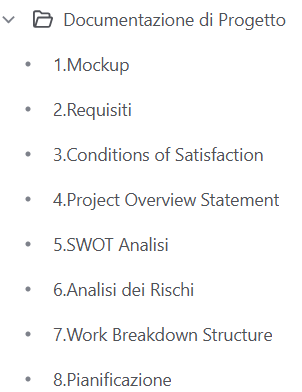
\includegraphics[scale=0.6]{figures/strutturaConfluenceProposta.png}
    \caption{Esempio di struttura della cartella relativa alla documentazione di progetto}
    \label{fig:doc-progetto}
\end{figure}

Per la gestione del \textbf{Project Management Life Cycle}, si consiglia un approccio Agile \cite{project2017agile}
\cite{sliger2008software} \cite{Peters20241} \cite{beck2001agile} \cite{wysocki2011effective}
iterativo basato su Kanban, poiché garantisce
la flessibilità necessaria per il metodo di sviluppo di \textit{Peer Network}, oltre ad adattarsi al rilascio dei moduli.
Inoltre, Kanban è il framework utilizzato all’interno di Jira, strumento già utilizzato per l’organizzazione del lavoro. L’obiettivo è
completare i moduli nel minor tempo possibile, cercando di anticipare le date concordate per i vari rilasci. Parallelamente, si
punta a coinvolgere maggiormente il cliente nei test, favorendo un ciclo di feedback continuo. Per queste ragioni,
l’adozione di un metodo di gestione tradizionale non risulterebbe adeguata. Il framework Scrum è stato utilizzato in passato su progetti di
grandi dimensioni, gestiti da project manager diversi, seguendo scrupolosamente tutte le indicazioni previste dalla metodologia.
Tuttavia, l’esperienza ha evidenziato alcune criticità: la produzione di documentazione all’inizio e alla fine di ogni sprint,
insieme alle retrospettive con il cliente, ha richiesto un impegno eccessivo, sottraendo tempo prezioso allo sviluppo effettivo.
Entrambi i project manager hanno quindi ritenuto che lo sforzo non fosse giustificato dai benefici ottenuti. Inoltre, l’adozione
di Scrum è stata possibile solo con quegli specifici clienti, poiché erano disposti a partecipare attivamente a frequenti riunioni di
allineamento. La maggior parte degli altri committenti, invece, preferisce un approccio meno coinvolgente, ritenendo che, una volta
commissionato un sistema, debba essere l’azienda sviluppatrice a gestire completamente il progetto senza richiedere un’interazione
continua. Questo rende Scrum difficilmente applicabile nel contesto operativo di \textit{Peer Network}.

    \subsection{Idea, Design, Economics}
    Attualmente, la politica aziendale prevede di accettare tutti i progetti che i clienti propongono,
    senza una valutazione approfondita delle eventuali
    criticità e accelerando la fase iniziale per avviare rapidamente lo sviluppo. Tuttavia, un'analisi più dettagliata
    consentirebbe di raccogliere informazioni più precise, ottimizzando le fasi successive del progetto.

        \paragraph{Ridefinizione dei ruoli}
        Si propone che il CEO assuma il ruolo di responsabile commerciale dell’azienda, intervenendo come supporto in altri aspetti
        solo quando necessario. Di conseguenza, l’analisi e la progettazione delle soluzioni dovranno essere affidate a un altro
        dipendente, da individuare, formare e affiancare fino al raggiungimento della piena autonomia nel ruolo. Inoltre, è
        essenziale coinvolgere il project manager sin dalle prime fasi, poiché ha la responsabilità di garantire il successo
        del progetto e il pieno soddisfacimento delle richieste del cliente.

        \paragraph{Riunioni con clienti}
        Durante gli incontri con i clienti, è importante coinvolgere il CEO, il project manager e l'analista/progettista.
        Questo approccio consente di raccogliere informazioni più dettagliate, assicurando che tutto ciò che viene discusso
        venga annotato con precisione. Inoltre, la presenza del project manager permette al cliente di conoscere direttamente
        la figura con cui collaborerà, facilitando la comunicazione e la gestione del progetto. Infine, il project manager
        può ascoltare in prima persona le esigenze del cliente, evitando il rischio di informazioni filtrate o distorte da intermediari.

        \paragraph{Requisiti}
        È fondamentale redigere in modo chiaro e dettagliato tutti i requisiti funzionali e non funzionali del sistema. Questo
        compito spetta a chi partecipa alle riunioni con il cliente, aggiornando l’elenco progressivamente man mano che emergono
        nuove informazioni e vengono chiariti i vari aspetti del progetto.
        I requisiti funzionali definiscono le caratteristiche essenziali del sistema, ovvero le operazioni e le funzionalità che
        deve svolgere per garantire il corretto funzionamento.
        I requisiti non funzionali, invece, riguardano aspetti come prestazioni, affidabilità, sicurezza e usabilità,
        influenzando il modo in cui il sistema opera e risponde alle esigenze del cliente, migliorandone l’efficienza complessiva.

        \paragraph{Condizioni di soddisfazione}
        Le condizioni di soddisfazione sono un elenco di criteri che definiscono quando il progetto è considerato completato,
        con obiettivi chiari e specifici. Devono essere redatte all'inizio del progetto e aggiornate alla fine, per garantire
        che tutte le aspettative siano state soddisfatte. Nella Figura \ref{fig:cond-sodd} è illustrato un esempio di come poter strutturare
        le condizioni e la loro descrizione in una tabella.
        \begin{figure}
            \centering
            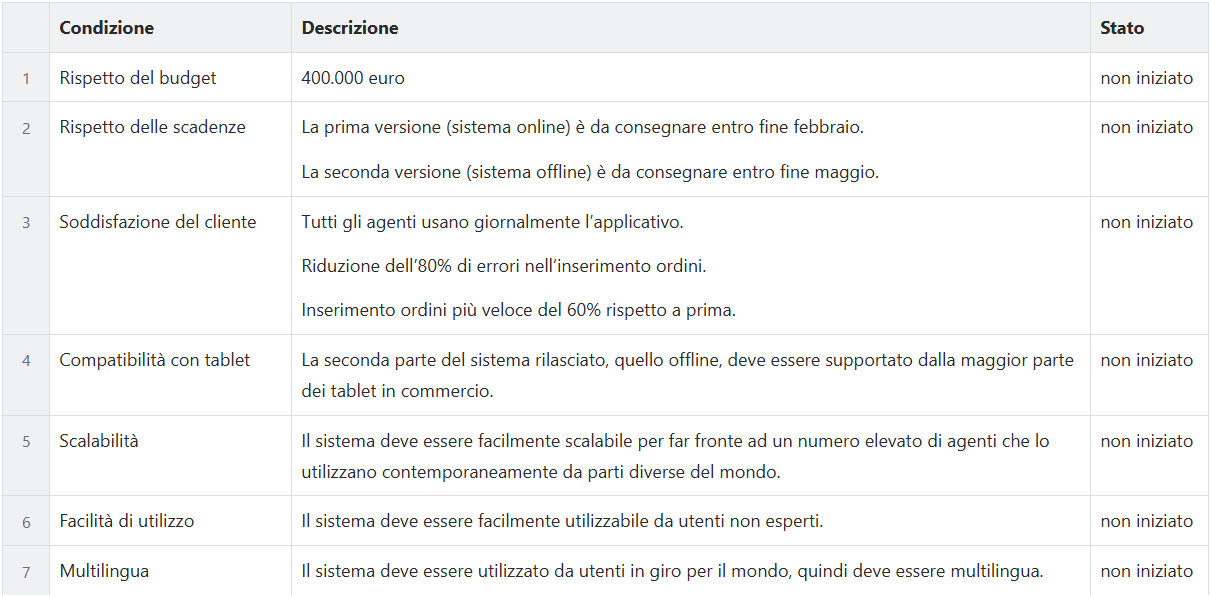
\includegraphics[width=\linewidth]{figures/CoS.png}
            \caption{Elenco delle condizioni di soddisfazione di progetto}
            \label{fig:cond-sodd}
        \end{figure}

        \paragraph{Project Overview Statement}
        Prima di redigere il contratto, è essenziale predisporre un documento da allegare, così da fornire al cliente una chiara
        visione di ciò che verrà realizzato. Questo materiale sarà il riferimento sia per il team che per il cliente, delineando
        l’intero progetto. Inoltre, sarà un supporto utile nelle decisioni future e nel processo di approvazione. La struttura proposta include:
        \begin{itemize}
            \item problema/opportunità: descrizione del motivo che giustifica il progetto, evidenziando il problema da risolvere o l'opportunità da cogliere;
            \item goal del progetto: spiegazione in modo chiaro e conciso dell'obiettivo principale del progetto;
            \item obiettivi: elenco dei traguardi specifici secondo il criterio SMART (Specifici, Misurabili, Assegnabili, Realistici, Temporizzati);
            \item criteri di successo: definizione delle metriche per valutare se il progetto avrà raggiunto i risultati desiderati;
            \item assunzioni: spiegazione delle condizioni considerate vere, ma non verificabili in modo diretto;
            \item rischi: descrizione di eventi o circostanze che potrebbero avere un impatto negativo sul progetto;
            \item ostacoli: elenco di eventuali barriere o limitazioni che potrebbero ostacolare il completamento del progetto.
        \end{itemize}

    \subsection{Progetto Software}
        \subsubsection{Avvio}
            \paragraph{Riunione di allineamento}
            La riunione ha l’obiettivo di introdurre e allineare il team leader. Sono
            presenti il project manager e il team leader; per i progetti di durata superiore alle tre settimane, partecipa
            anche il cliente.
            Durante l’incontro, vengono presentati i principali documenti di riferimento, tra cui i requisiti, i mockup,
            il Project Overview Statement e le Conditions of Satisfaction. Inoltre, il team leader riceve una panoramica
            dettagliata del progetto, così da comprendere il contesto, gli obiettivi e le aspettative, facilitando il
            suo inserimento e il coordinamento operativo.

            \paragraph{Riunioni operative interne}
            Alle riunioni operative interne partecipano il project manager e il team leader, mentre, per progetti
            complessi di durata superiore alle tre settimane, è coinvolta anche una figura interna con esperienza
            per un supporto aggiuntivo. Durante questi incontri, vengono condotte analisi strutturate come l'analisi SWOT
            e l’analisi dei rischi, per identificare punti di forza, debolezze, opportunità e minacce legate al progetto.
            Le discussioni si basano sui documenti prodotti in precedenza.

            \begin{figure}
                \centering
                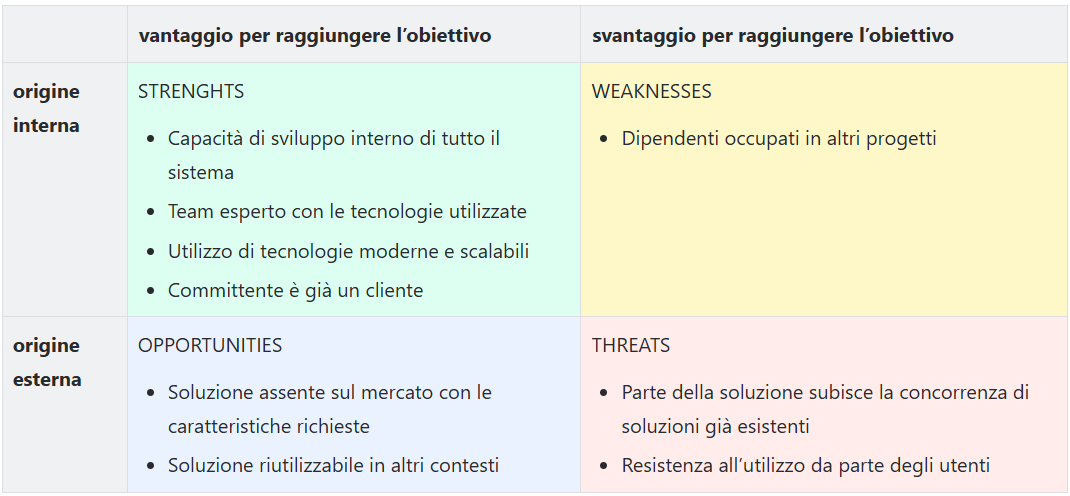
\includegraphics[width=\linewidth]{figures/swot.png}
                \caption{Schema raffigurante l'analisi SWOT}
                \label{fig:swot}
            \end{figure}
            \paragraph{Analisi SWOT}
            L'analisi SWOT consente di valutare i fattori interni ed esterni che possono influenzare il successo di un progetto.
            Questa analisi aiuta a comprendere meglio il contesto in cui si opera, consentendo di elaborare strategie mirate
            per sfruttare i punti di forza e le opportunità, riducendo al minimo debolezze e minacce. Viene riportata in Figura \ref{fig:swot}
            una possibile struttura, ricreabile facilmente in un documento di Confluence. Si suddivide in quattro categorie principali:
            \begin{itemize}
                \item strengths (punti di forza): fattori interni che rappresentano un vantaggio competitivo. Possono includere
                competenze tecniche avanzate, un team esperto, una clientela fidelizzata o l’utilizzo efficace di una tecnologia specifica;
                \item weaknesses (debolezze): aspetti interni che possono ostacolare il raggiungimento degli obiettivi. Esempi
                tipici sono la mancanza di risorse, la scarsa esperienza su una tecnologia, una gestione disorganizzata o carenze nel team;
                \item opportunities (opportunità): elementi esterni che possono favorire il progetto. Tra questi rientrano l’accesso a
                un mercato poco competitivo, nuove normative vantaggiose o l’emergere di esigenze specifiche da parte dei clienti;
                \item threats (minacce): fattori esterni che potrebbero rappresentare un rischio. Alcuni esempi sono l’ingresso di
                nuovi competitor, cambiamenti normativi sfavorevoli, scarsa accettazione da parte degli utenti o recensioni negative.
            \end{itemize}

            \begin{figure}
                \centering
                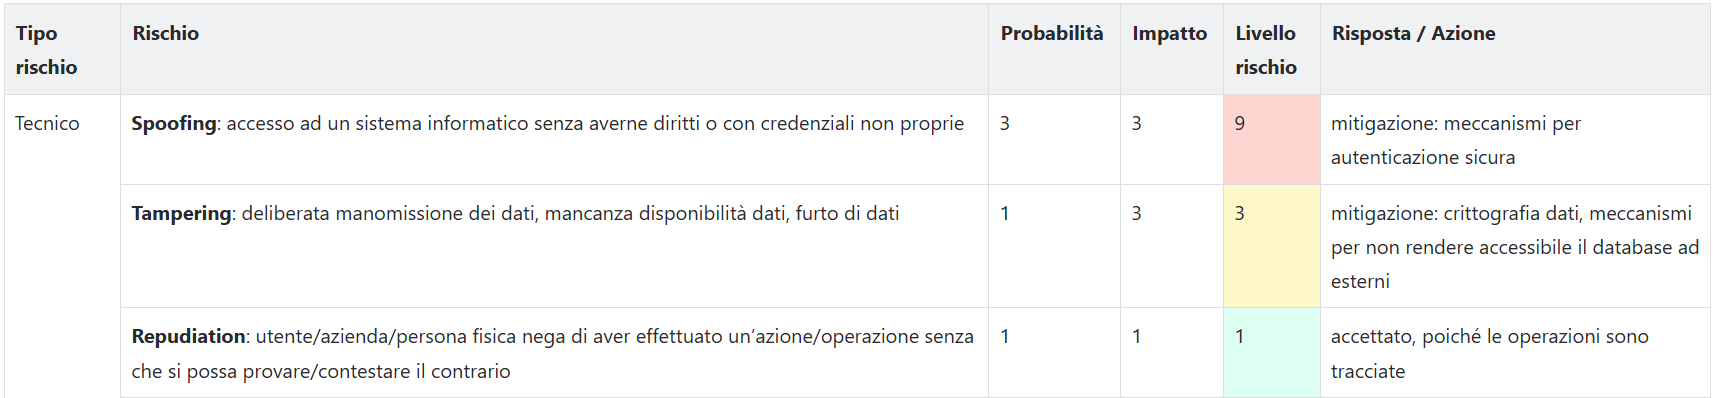
\includegraphics[width=\linewidth]{figures/risks.png}
                \caption{Parte dell'analisi dei rischi tecnici}
                \label{fig:risks}
            \end{figure}
            \paragraph{Analisi rischi}
            L’analisi dei rischi è necessaria per individuare le possibili criticità e definire strategie di mitigazione o prevenzione.
            Inoltre, risulta fondamentale per stabilire il livello di sicurezza tecnica da applicare, in linea con l’obiettivo
            aziendale di rafforzare la sicurezza delle proprie soluzioni. Questo processo deve coinvolgere più persone, così da
            confrontare idee e trovare un punto d’incontro.
            L’analisi dei rischi si articola in tre fasi principali: identificazione, valutazione e definizione delle azioni correttive.
            Successivamente, durante lo sviluppo, sarà essenziale implementare un sistema di monitoraggio e controllo per garantire
            la gestione continua delle vulnerabilità.

            L’approccio seguito parte dall'analisi SWOT, per poi stilare tutti i rischi e classificarli
            in quattro categorie principali: tecnici, project management, organizzativi ed esterni.
            Per rendere l’analisi più intuitiva ed efficace, le informazioni vengono organizzate all’interno di una tabella strutturata,
            una parte raffigurata in Figura \ref{fig:risks}.
            Ogni elemento viene classificato in base alla tipologia e valutato considerando la probabilità di accadimento, l’impatto
            e il livello di criticità, indicando anche le azioni correttive da adottare per limitarne le conseguenze.
            La determinazione del livello di gravità può avvenire attraverso una matrice specifica, mostrata in Figura \ref{fig:risk-matrix},
            che permette di identificare
            immediatamente la criticità in base alla combinazione tra probabilità e impatto. In alternativa, è possibile utilizzare
            un sistema numerico assegnando valori progressivi: 1 per bassa rilevanza, 2 per media e 3 per alta. Il punteggio
            complessivo si ottiene moltiplicando i due fattori e classificando il risultato secondo tre fasce di rischio:
            basso (1-2), medio (3-4) e alto (6-9).

            Per affrontare i rischi tecnici di sicurezza, \textit{Peer Network} ha deciso di adottare le linee guida di Intesys\footnote{\url{https://www.intesys.it/information-technology/metodologia-e-approccio/sviluppo-codice-sicuro/}}
            descritte nel documento “Sviluppo di codice sicuro”. In questo contesto, viene utilizzato il modello STRIDE,
            sviluppato da Microsoft, per identificare e classificare le principali minacce alla sicurezza di un sistema.
            Questo framework suddivide le vulnerabilità in sei categorie: Spoofing, Tampering, Repudiation, Information
            Disclosure, Denial of Service ed Elevation of Privilege, coprendo un’ampia gamma di potenziali problemi.
            In quest’ottica, l’azienda sta iniziando a definire un piano di sicurezza informatica basato su tre livelli:
            \begin{itemize}
                \item base: applicato a tutti i sistemi senza distinzioni;
                \item medio e alto: definiti in base alle specifiche esigenze di sicurezza.
            \end{itemize}

            \begin{figure}
                \centering
                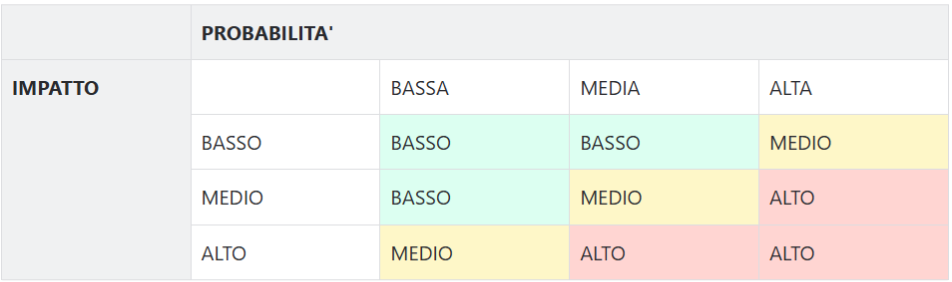
\includegraphics[scale=0.5]{figures/riskMatrix.png}
                \caption{Matrice del rischio}
                \label{fig:risk-matrix}
            \end{figure}

            \paragraph{Gestione risorse}
            Per garantire il successo del progetto, è fondamentale analizzare e pianificare con precisione le risorse necessarie. Questa fase comprende:
            \begin{itemize}
                \item risorse umane: definizione dei membri del team coinvolti nel progetto e registrazione delle assegnazioni in un documento dedicato all'interno dello spazio Confluence;
                \item costi e budget: utilizzo del business case automatizzato su \ac{PAM} (dettagliato nel Capitolo \ref{chap:pam}) per monitorare i costi,
                i ricavi e i margini, sia in fase di pianificazione che a progetto avviato.
            \end{itemize}

            \paragraph{Project Definition Statement}
            Questo documento, rivolto al team, arricchisce il Project Overview Statement con una descrizione approfondita
            del progetto. Oltre a definire chiaramente le attività da svolgere, fornisce linee guida per mantenere la concentrazione
            sugli obiettivi. Include inoltre dettagli sull’approccio di sviluppo e sulle specifiche tecniche e operative, offrendo
            un quadro completo del lavoro da eseguire.

        \subsubsection{Pianificazione}
            \paragraph{Riunioni operative interne}
            Le riunioni operative interne coinvolgono il project manager, il team leader e, per progetti superiori alle tre
            settimane, anche le figure con esperienza. Durante questi incontri, il gruppo lavora per scomporre il
            progetto in attività più dettagliate, creando una \ac{WBS} di livello logico. Successivamente,
            si procede con la stima della durata delle singole attività e l’identificazione delle dipendenze tra di esse.
            Infine, si pianifica il progetto delineando le scadenze generali per il
            rilascio dei vari moduli, utilizzando strumenti come il diagramma di Gantt e Jira per mantenere una chiara visione d’insieme.
            
            \begin{figure}
                \centering
                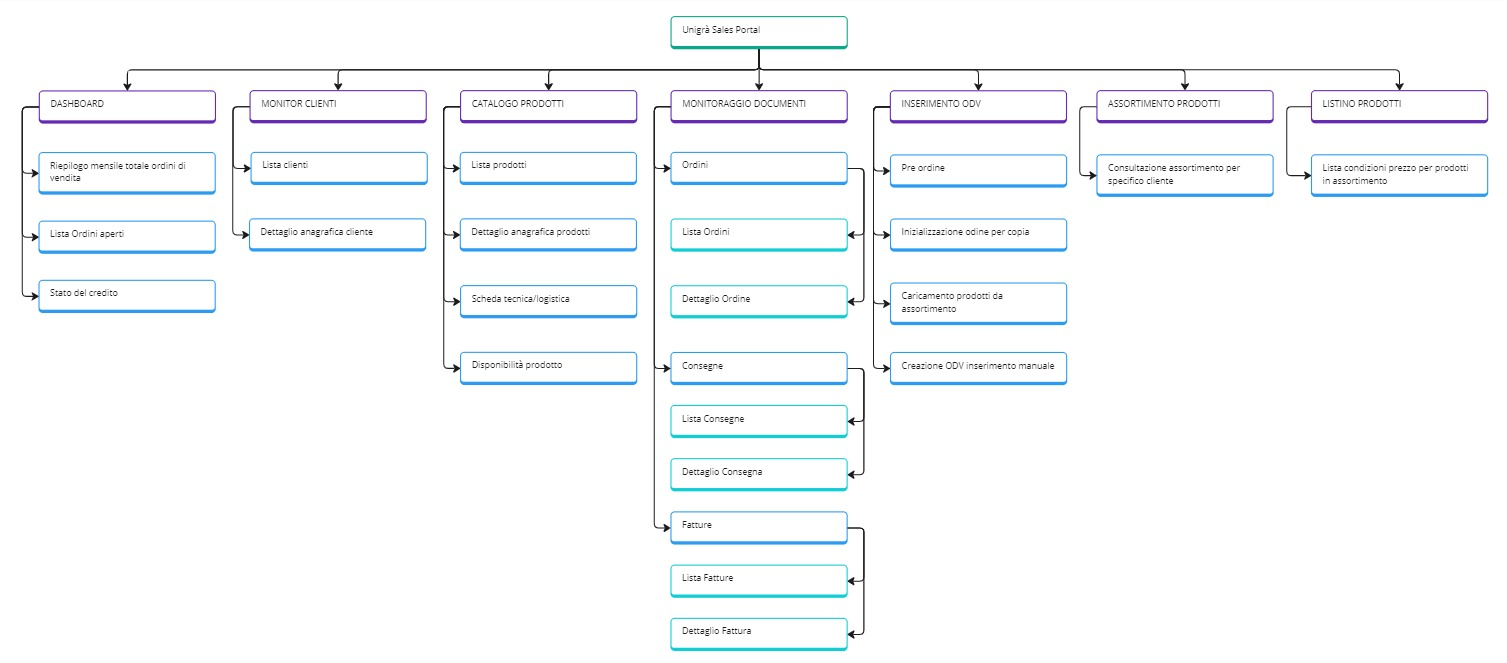
\includegraphics[width=\linewidth]{figures/ProgettoClienteWBS.jpg}
                \caption{Struttura logica di un progetto cliente, schematizzata in una WBS}
                \label{fig:wbs-nuovo}
            \end{figure}
            \paragraph{Work Breakdown Structure}
            La \ac{WBS} è una rappresentazione gerarchica delle attività necessarie per completare il progetto, così da
            soddisfare i criteri di successo richiesti dal committente. Essendo uno
            strumento iterativo, può essere affinato progressivamente e non è necessario definirlo completamente all’inizio.

            Si utilizza una struttura ad albero per offrire una visione d’insieme chiara e immediata. La scomposizione del
            problema avviene partendo dai mockup e modellando il dominio a livello logico. La \ac{WBS} è articolata su tre livelli:
            \begin{itemize}
                \item livello 1 (elementi in viola): rappresenta i moduli principali in cui si suddivide il progetto;
                \item livello 2 (elementi in azzurro): identifica le funzionalità richieste per ciascun modulo;
                \item livello 3 (elementi in azzurro acqua): offre un’ulteriore suddivisione delle funzionalità.
            \end{itemize}
            È fondamentale concordare con il cliente quali moduli sviluppare, specificandone le funzionalità e definendo
            l'ordine di implementazione. In Figura \ref{fig:wbs-nuovo} è riportato un esempio di \ac{WBS} per un progetto cliente,
            realizzata tramite lo strumento Miro.

            \begin{figure}
                \centering
                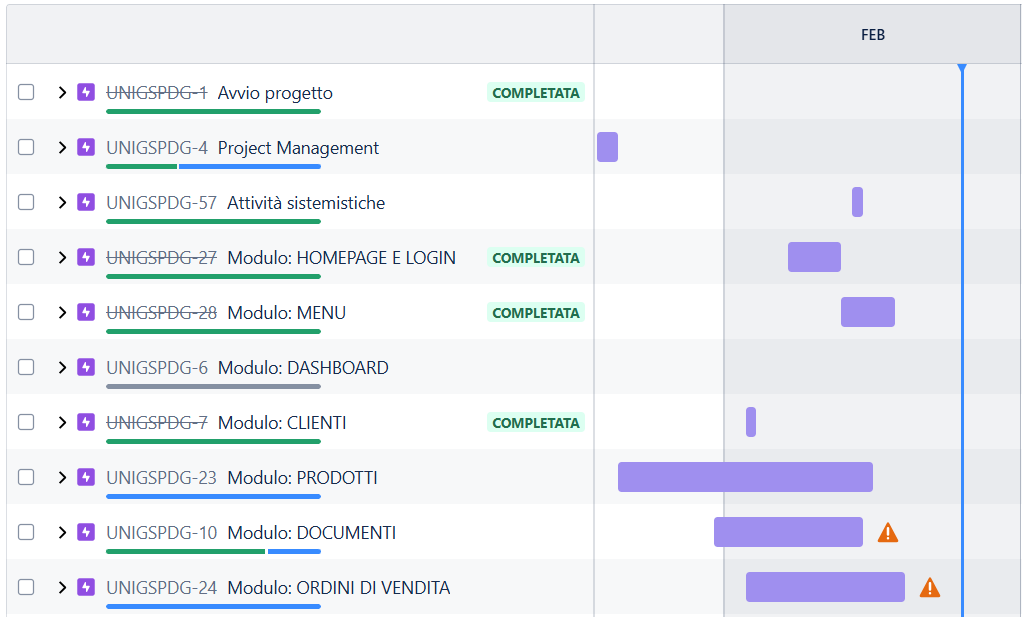
\includegraphics[scale=0.6]{figures/timelineJiraNuovo.png}
                \caption{Pianificazione temporale di un progetto su Jira}
                \label{fig:timeline-nuovo}
            \end{figure}
            \paragraph{Pianificazione generale nel Gantt}
            Il diagramma di Gantt consente di visualizzare in modo chiaro la pianificazione di un progetto, evidenziando
            attività, scadenze e relazioni tra le varie fasi. Inizialmente, la struttura del progetto viene definita a
            livello logico su Gantt, per poi essere implementata su Jira. Per la creazione del diagramma si può ricorrere
            a GanttPro, ma un’alternativa valida è sfruttare la Timeline di Jira, organizzando la pianificazione sulle epic,
            così da mantenere l’intero processo all’interno della stessa piattaforma (esempio in Figura \ref{fig:timeline-nuovo}).

            \begin{figure}
                \centering
                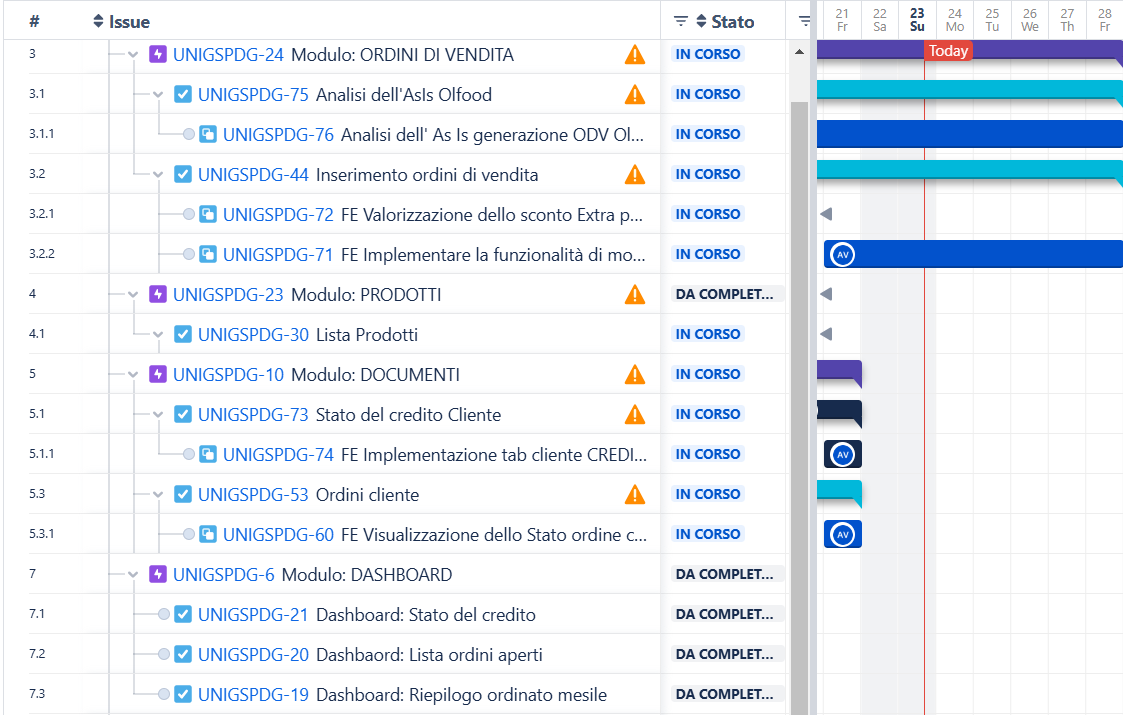
\includegraphics[scale=0.6]{figures/GanttJiraNuovo.png}
                \caption{Struttura gerarchica su Jira delle attività di progetto}
                \label{fig:gantt-nuovo}
            \end{figure}
            \paragraph{Pianificazione attività in Jira}
            Per pianificare le attività su Jira (Figura \ref{fig:gantt-nuovo}), le nuove linee guida aziendali stabiliscono quanto segue:
            \begin{itemize}
                \item livello logico (responsabile: project manager):
                \begin{itemize}
                    \item epic (livello 1 dalla \ac{WBS}, colore viola): per ogni epic, va allegato come descrizione il link
                    al documento Confluence che ne dettaglia i contenuti, centralizzando tutta la documentazione;
                    \item task (livello 2 dalla \ac{WBS} o livello 3 se presente, colore azzurro): ciascun task dovrà avere
                    una descrizione dettagliata o un link ai documenti Confluence utili. Questa parte può essere affinata
                    iterativamente anche poco prima dell'inizio dello sviluppo, sebbene sia preferibile avere già ben chiare le attività principali da sviluppare.
                \end{itemize}
                \item livello tecnico (responsabile: team leader):
                \begin{itemize}
                    \item subtask: attività operative. Ogni subtask dovrà essere corredato da una descrizione dettagliata o da un
                    link ai documenti di riferimento, con la possibilità di essere perfezionato settimanalmente o dopo il rilascio di un modulo precedente.
                \end{itemize}
            \end{itemize}

            Durante la pianificazione generale, è fondamentale stimare approssimativamente la durata delle attività relative alle epic e ai task,
            identificando le dipendenze tra le attività per stabilirne le priorità.

            \paragraph{Riunione allineamento con cliente}
            La riunione di allineamento con il cliente coinvolge il project manager, il team leader e il cliente stesso.
            Durante l'incontro, viene presentata la \ac{WBS}, che illustra la scomposizione del progetto. Successivamente,
            si discute la pianificazione del progetto, comprese le scadenze tramite il Gantt, per fornire una visione
            chiara del cronoprogramma delle attività. L'incontro si conclude con una discussione, eventuali modifiche e
            la validazione di quanto presentato, per garantire che il piano sia allineato con le aspettative e le esigenze del cliente.

        \subsubsection{Esecuzione}
            \paragraph{Programmazione attività settimanali}
            Ogni venerdì il team leader raffina i task e dettaglia le attività operative dei subtask all'interno di Jira. In questa fase,
            egli stima la durata di ciascun compito e successivamente assegna il subtask allo
            sviluppatore responsabile dell'esecuzione. Questo processo consente di garantire un monitoraggio accurato e un'efficace gestione
            delle attività settimanali.

            \paragraph{Selezione membri team di progetto}
            La selezione dei membri del team per il progetto avviene in base alle attività operative identificate in precedenza.
            La decisione sui ruoli e sulle persone da coinvolgere nello sviluppo dipende dalle competenze richieste per ciascuna attività specifica.

            \paragraph{Riunione allineamento team completo}
            La riunione di allineamento del team completo viene convocata solo se ci sono sviluppatori che non sono stati coinvolti fino a
            quel momento. Durante l'incontro, si presenta l'intero progetto utilizzando tutto il materiale prodotto in precedenza. Tutti i
            membri del team di progetto partecipano a questa riunione per garantire che siano allineati e informati sugli sviluppi.

            \paragraph{Piano di qualità}
            Il piano qualità del lavoro deve essere condiviso con tutto il team, che deve seguirlo rigorosamente.
            Gli aspetti principali sono:
            \begin{itemize}
                \item codice manutenibile: è fondamentale organizzare una riunione per spiegare le linee guida, che comprendono aspetti
                come convenzioni sui commit, la denominazione dei branch o l'importanza dei commenti nel codice;
                \item sicurezza software: bisogna applicare le linee guida di sicurezza stabilite da Intesys, garantendo che tutte
                le pratiche siano seguite correttamente;
                \item documentazione di progetto: i file di progetto su Confluence devono essere costantemente aggiornati, in modo che tutti
                abbiano accesso alle informazioni più recenti;
                \item documentazione del codice:
                \begin{itemize}
                    \item Javadoc per esterni: ogni funzione e file devono essere corredati da una descrizione in inglese che spieghi
                    il funzionamento del codice, i parametri in input e i valori restituiti.
                    Queste informazioni devono seguire lo standard Javadoc\footnote{\url{https://www.oracle.com/java/technologies/javase/javadoc-tool.html}};
                    \item commenti interni nel codice: è importante includere spiegazioni dettagliate delle logiche più complesse
                    direttamente nel codice, per facilitare la comprensione da parte di chi dovrà modificarlo in futuro.
                \end{itemize}
                \item test automatici: devono essere implementati alcuni tipi di test automatici per semplificare la validazione
                del progetto durante tutti i rilasci dei moduli, in vista della fase finale di rilascio, approfondita successivamente.
            \end{itemize}

            \paragraph{Regole per la comunicazione}
            Le seguenti regole di comunicazione devono essere condivise con tutto il team e seguite da ogni membro:
            \begin{itemize}
                \item riunioni di progetto:
                \begin{itemize}
                    \item le riunioni periodiche devono essere programmate con frequenza variabile, a seconda delle esigenze del progetto;
                    \item project review meeting: questi incontri si tengono ogni volta che viene rilasciato un modulo del progetto.
                    Devono partecipare il project manager e gli sviluppatori, così da confrontarsi sul lavoro svolto e l'organizzazione utilizzata.
                \end{itemize}
                \item monitoraggio di criticità e problemi: ogni volta che si presenta un problema, deve essere documentato in Confluence,
                inserito in una tabella e seguito da un confronto: se il problema è di entità minore, il team può discuterne in riunioni
                interne; mentre, se il problema è significativo, il project manager deve avviare un incontro con il committente, dato che
                la decisione finale dipende dal cliente;
                \item gestione delle comunicazioni:
                \begin{itemize}
                    \item documentazione di progetto: deve essere creata e aggiornata costantemente su Confluence, dove tutti i membri
                    del team possono modificarla e visualizzarla facilmente;
                    \item comunicazione tra sviluppatore e project manager: se emergono problemi o questioni aperte, devono essere
                    segnalati nella sezione commenti del relativo subtask su Jira, in modo che il project manager possa tenere
                    traccia di ogni dettaglio. Inoltre, è fondamentale che i membri del team aggiornino tempestivamente lo stato
                    dei subtask per avere sempre una visione chiara dell’avanzamento del lavoro;
                    \item comunicazione tra project manager e direzione: ogni settimana, il project manager deve aggiornare il report
                    riassuntivo del progetto, includendo le date dei rilasci e le informazioni utili per monitorare lo stato
                    generale del progetto. Questo non solo aiuta la direzione, ma anche il project manager a mantenere una visione
                    d'insieme delle attività completate e di quelle future. Inoltre, consente a tutti i project manager di monitorare
                    lo stato globale dei progetti, facilitando la gestione delle tempistiche e la pianificazione degli sforzi, in
                    particolare per evitare conflitti nelle date di rilascio quando ci sono più progetti in corso.
                \end{itemize}
            \end{itemize}
        
        \subsubsection{Rilascio}
            \paragraph{Test automatici}
            Alcuni tipi di test che potrebbero essere inseriti, in base alla tipologia di soluzioni sviluppate dall’azienda:
            \begin{itemize}
                \item regressione: per verificare che nuove modifiche al software, come aggiornamenti o correzioni di bug, non abbiano
                introdotto errori in altre parti del sistema;
                \item prestazioni: valutano la velocità, la stabilità e la scalabilità del software sotto diverse condizioni di carico;
                \item sicurezza: progettati per individuare vulnerabilità all’interno del software, garantendo che i dati sensibili siano
                protetti e che il sistema sia resistente a potenziali attacchi;
                \item integrazione: verificano che i diversi moduli o componenti del software funzionino correttamente insieme.
            \end{itemize}
            
            \paragraph{Riunioni di retrospettiva post-installazione completata}
            Al termine dello sviluppo di un sistema e dell'installaizione finale presso il cliente, sarebbe importante svolgere:
            \begin{itemize}
                \item una riunione interna: l'incontro serve per analizzare insieme cosa ha funzionato bene e cosa può essere migliorato,
                in modo da ottimizzare i processi per i futuri progetti;
                \item una riunione con il cliente: dopo alcune settimane di utilizzo del sistema, è importante raccogliere pareri
                per verificare se il progetto soddisfa le
                esigenze richieste, identificando gli aspetti positivi e le eventuali aree che richiedono miglioramenti.
            \end{itemize}           

    \subsection{Supporto e Servizio}
    Il lavoro del team di supporto dovrebbe risultare più semplice grazie alle migliorie introdotte nelle fasi precedenti.
    La manutenzione del codice è ottimizzata, la documentazione tecnica e di progetto è aggiornata e il codice stesso
    è corredato da commenti chiari, garantendo così una gestione più efficiente e strutturata.
    

\chapter{Peer Network Activity Management}
\label{chap:pam}

Il sistema \textbf{\ac{PAM}} è stato il primo progetto in cui sono state
adottate le \ac{PBC}, segnando una svolta importante nel modo di sviluppare le applicazioni in \textit{Peer Network}.
In precedenza, l’infrastruttura della piattaforma di integrazione \ac{ESI}, che accoglie al suo interno
le \ac{PBC}, seguiva un’architettura monolitica. Tuttavia, l’implementazione di \ac{PAM} ha offerto un contesto
ideale per sperimentare e testare questa nuova metodologia. Il successo ottenuto
durante questa fase sperimentale ha dimostrato l’efficacia delle \ac{PBC}, non solo nel migliorare la
flessibilità e modularità del sistema, ma anche nel semplificare i processi di sviluppo. Questo ha
portato alla decisione strategica di estendere l’approccio basato sulle \ac{PBC} a tutte le
\ac{SBS} progettate successivamente per i clienti, segnando un’evoluzione
significativa nell’architettura delle applicazioni aziendali.

In questo capitolo vengono approfonditi i concetti introdotti precedentemente, riguardanti
le applicazioni componibili e le \ac{PBC}. Verrà esaminato come \textit{Peer Network} abbia
adottato e adattato questi principi nello sviluppo delle proprie \ac{SBS}, analizzandone la struttura
generale e il funzionamento. Successivamente, l’attenzione sarà focalizzata su \ac{PAM}, che rappresenta un
caso specifico di \ac{SBS}. Poiché \ac{PAM} e le \ac{SBS} condividono la stessa architettura strutturale basata sulle
\ac{PBC}, il sistema sarà utilizzato come esempio pratico per illustrare l’applicazione concreta di tali
concetti.

\section{Struttura di una Smart Business Solution}
La \textit{Peer Network} ha sviluppato gli schemi riportati in Figura \ref{fig:sbs} e Figura \ref{fig:sbs-sap}
per illustrare, all'interno della propria comunicazione, l’organizzazione delle applicazioni componibili che realizza.
Queste, denominate \ac{SBS}, sono progettate per clienti appartenenti a diversi settori.
Ciascuna soluzione è composta da:
\begin{itemize}
    \item componenti backend, che integrano servizi e dati distribuiti su più piattaforme. Questa parte
    comprende inoltre la piattaforma di integrazione \ac{ESI}, responsabile della gestione delle \ac{PBC}
    necessarie;
    \item componenti frontend, sviluppati e successivamente distribuiti tramite la piattaforma Liferay\footnote{\url{https://www.liferay.com/it/home}}.
\end{itemize}

\begin{figure}
    \centering
    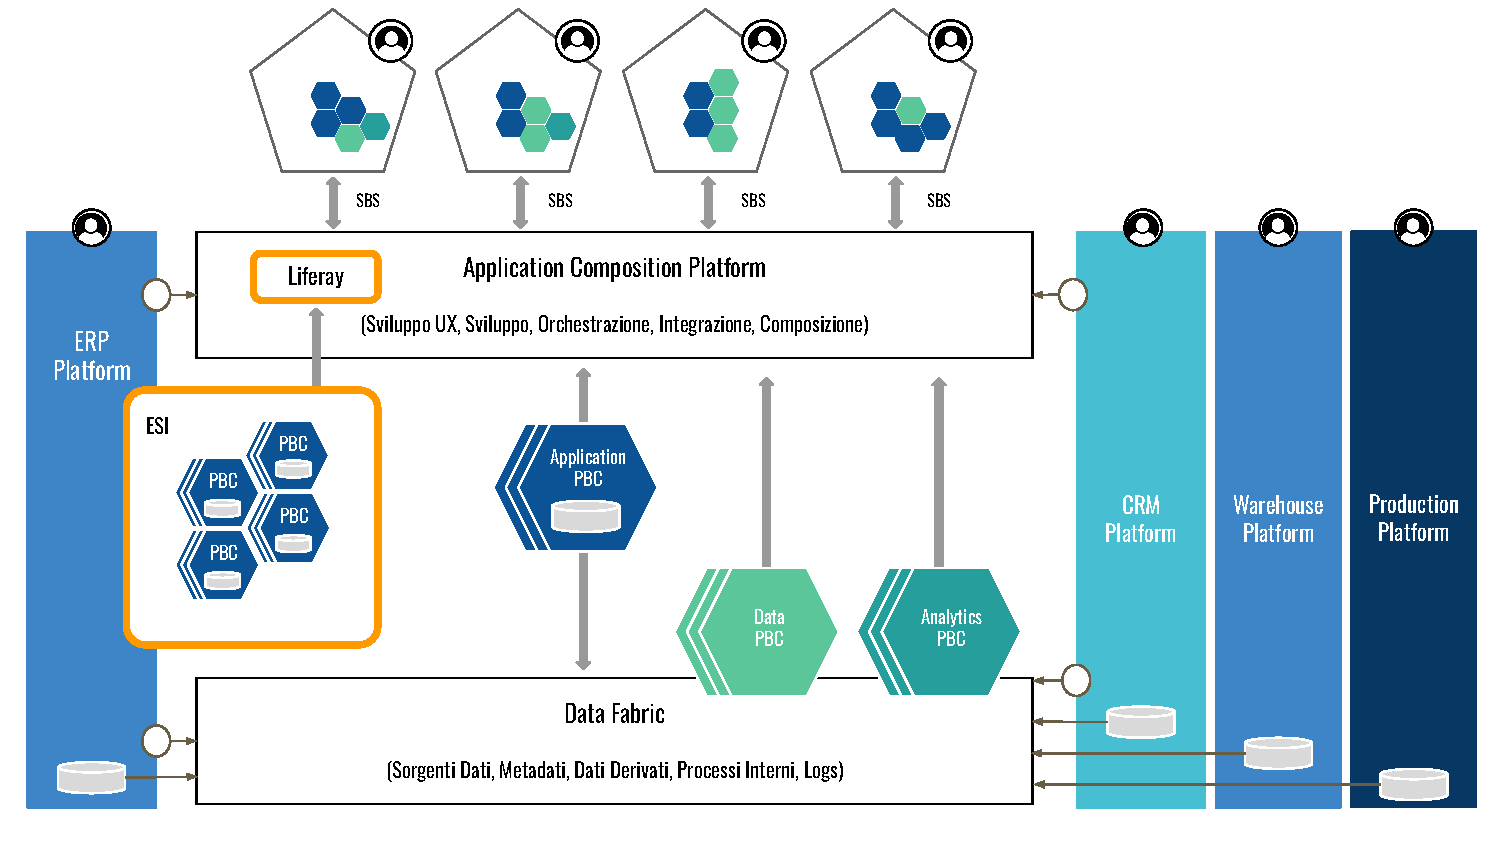
\includegraphics[width=\linewidth]{figures/struttura-sbs.pdf}
    \caption{Struttura di una SBS e interazione tra i vari sistemi integrati}
    \label{fig:sbs}
\end{figure}

Dal punto di vista tecnico, ogni \ac{SBS} è composta da:
\begin{itemize}
    \item una parte di \textbf{backend}, che gestisce le logiche applicative ed è suddivisa in:
        \begin{itemize}
            \item \textbf{livello Data Fabric}, include sistemi informativi aziendali o database con cui la
            \ac{SBS} interagisce: ad esempio, può trattarsi di un \ac{ERP} (es. SAP), di un sistema \ac{CRM}
            (es. Salesforce) o di un database relazionale (es. MySQL). Poiché la maggior parte
            dei clienti utilizza sistemi SAP, le soluzioni si distinguono principalmente in SAP e non-SAP. In Figura
            \ref{fig:sbs-sap}, questo livello è rappresentato nella versione SAP;
            \item \textbf{livello \ac{PBC} Repository}, piattaforma \textbf{\ac{ESI}}: composto da \ac{PBC}, che forniscono accesso
            ai relativi dati e logiche applicative presenti nel livello Data Fabric. Le \ac{PBC}, pubblicate
            dalla piattaforma \ac{ESI}, fungono da intermediari tra le applicazioni e i sistemi informativi aziendali.
            A differenza di quanto formalizzato da Gartner, che individuava tre
            elementi base di una \ac{PBC}, dato, logiche e UI (opzionale), le \ac{PBC} di \textit{Peer Network} non contengono
            le rispettive interfacce utente, garantendo indipendenza tecnologica dal frontend. Sono state
            considerate due tipologie di \ac{PBC}:
            \begin{itemize}
                \item core: coprono funzionalità comuni a qualsiasi applicazione e cliente, quindi
                sono presenti in ogni \ac{SBS}. Nella Figura \ref{fig:sbs-sap} sono rappresentate dai cubi blu
                del livello PBC Repository;
                \item custom: realizzate per esigenze specifiche e applicazioni dedicate. Nella Figura \ref{fig:sbs-sap} sono rappresentate dai cubi
                arancioni del livello PBC Repository.
            \end{itemize}
            Le \ac{PBC} sono implementate come microservizi scritti in Kotlin\footnote{\url{https://kotlinlang.org}} e distribuite come container
            Docker\footnote{\url{https://www.docker.com}}, ciascuno contenente un gruppo coerente di \ac{PBC}. Ad esempio, G02 MATERIALS è il gruppo con
            funzionalità relative ai materiali, come il tipo di materiale PBC 0208 MATTYPE, la lista dei
            prezzi dei materiali PBC 0217 MATPRICELIST e l’unità di misura dei materiali PBC 0222 UNITOFMEASURE.
            In uno scenario on-premise (installazione presso il data-center del cliente), i
            microservizi sono orchestrati tramite Docker Compose. In uno scenario on-cloud, i
            microservizi vengono gestiti tramite Kubernetes\footnote{\url{https://kubernetes.io}}.
        \end{itemize}
    \item una parte di \textbf{frontend} chiamata \textbf{Composable layer}: è dedicata all’esperienza utente, il quale interagisce con
    la soluzione attraverso un'applicazione web.
    Anche il frontend viene realizzato come un insieme di moduli componibili (chiamati portlet)
    scritti in JavaScript utilizzando il framework Vue.js. Le portlet vengono assemblate in pagine web
    pubblicate tramite Liferay, seguendo un approccio componibile. Anche il frontend è gestito come
    microservizi, installati e orchestrati con modalità analoghe al livello \ac{PBC} Repository, sia in
    ambienti on-premise che cloud.
\end{itemize}

\begin{figure}
    \centering
    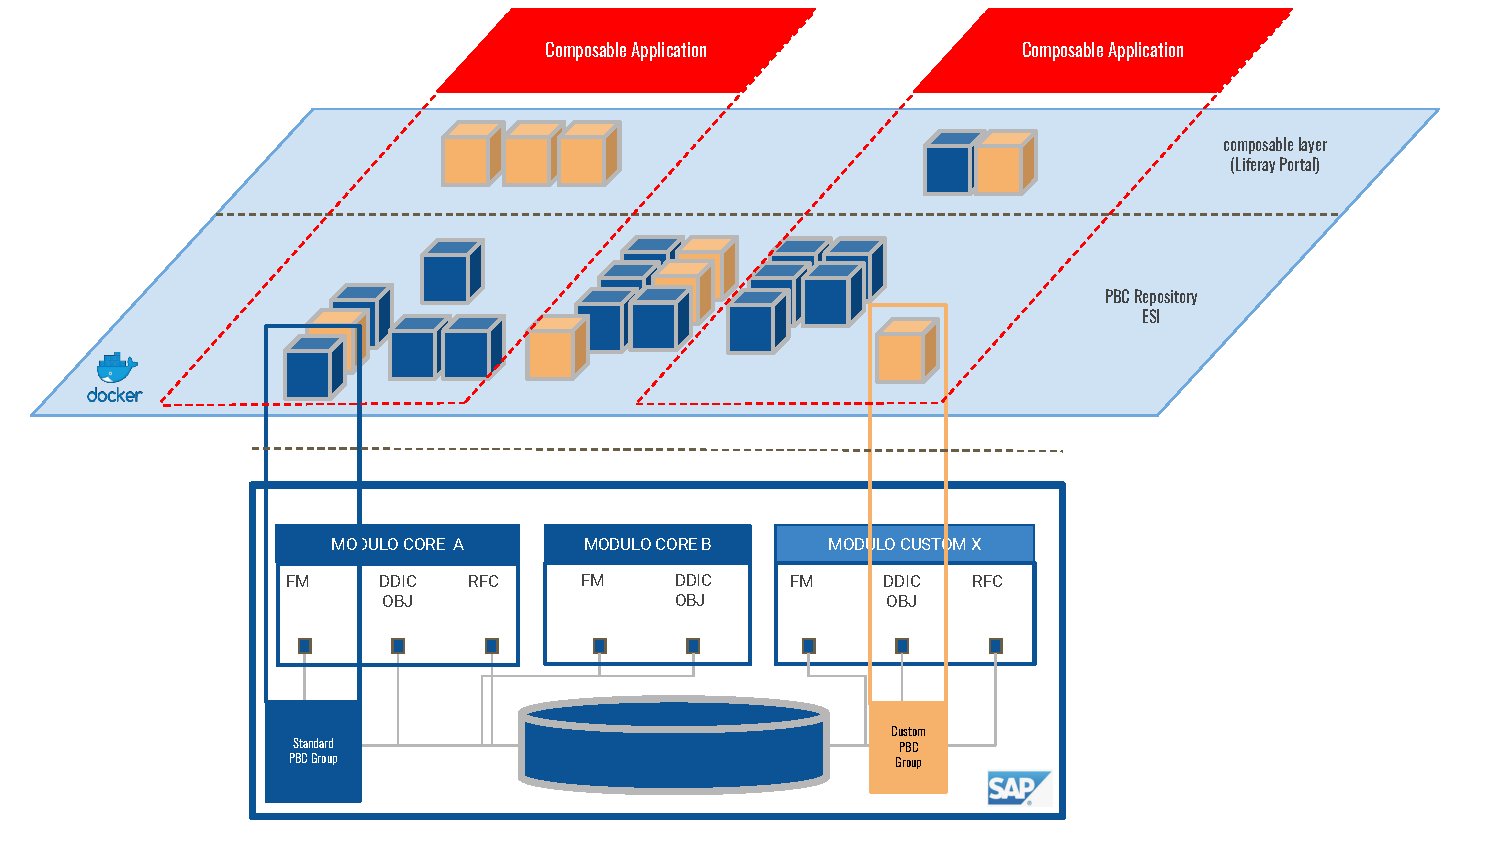
\includegraphics[width=\linewidth]{figures/architetturaSBS_SAP.pdf}
    \caption{Struttura di una SBS che interagisce con un ERP di SAP}
    \label{fig:sbs-sap}
\end{figure}

Entrando più nello specifico del livello \ac{PBC} Repository, la piattaforma \ac{ESI} gestisce le \ac{PBC}
attraverso due diversi livelli:
\begin{itemize}
    \item \textbf{livello API REST}: ospita i servizi di alto livello, cioè quelli riportati nella descrizione
    della \ac{PBC}. Questo strato è indipendente dallo scenario di implementazione ed è legato alla
    definizione dell’oggetto, così come la struttura dati;
    \item \textbf{livello sub-service}: ospita i servizi che interagiscono direttamente con lo strato dati
    della \ac{PBC}. I servizi implementati in questo livello differiscono a seconda del sistema informativo
    o database aziendale con il quale interagiscono:
    \begin{itemize}
        \item scenario SAP: i due layer API REST e sub-service sono gestiti da \ac{ESI} per SAP.
        In questo scenario, il sub-service layer è costituito da BAPI, RFC e FM, ovvero moduli di funzione SAP
        che consentono l'integrazione e l'interazione con l'\ac{ERP}, oltre a servizi REST che accedono alla base dati;
        \item scenario non-SAP: i due layer API REST e sub-service sono gestiti dalla versione
        di \ac{ESI} non-SAP. In questo scenario il sub-service layer è costituito da servizi che
        interagiscono con un database relazionale.
    \end{itemize}
\end{itemize}

    \subsection{Struttura di Peer Network Activity Management}
    Considerando l’architettura delle \ac{SBS} descritta in precedenza, quella di \ac{PAM} include:
    \begin{itemize}
        \item un modulo di backend che comprende:
        \begin{itemize}
            \item la base dati: come piattaforma per il database viene usato MySQL ed è installato presso il
            cloud provider OVH\footnote{\url{https://www.ovhcloud.com}} su una macchina proprietaria;
            \item le logiche che interagiscono con la base dati e i servizi relativi, viene usato
            \ac{ESI} non-SAP (installato presso il cloud provider OVH su una macchina proprietaria) come
            strumento di esposizione dei servizi e integrazione con le componenti di frontend.
        \end{itemize}
        \item un modulo di frontend che gestisce la UX/UI dell’applicazione, realizzato su
        Liferay Community Edition installato presso il cloud provider OVH su una macchina proprietaria.
    \end{itemize}

\section{Attività svolte}
Le attività di sviluppo hanno riguardato l’applicazione \ac{PAM}, un software utilizzato internamente all’azienda
per la gestione di aspetti organizzativi e burocratici. Il lavoro si è concentrato principalmente sullo
sviluppo frontend, utilizzando anche alcuni servizi esposti dalle \ac{PBC}, oltre ad un breve intervento
dedicato alla modifica di alcuni dati all'interno del database relazionale.

    \subsection{Sviluppo nell'area Progetti}
    \begin{figure}
        \centering
        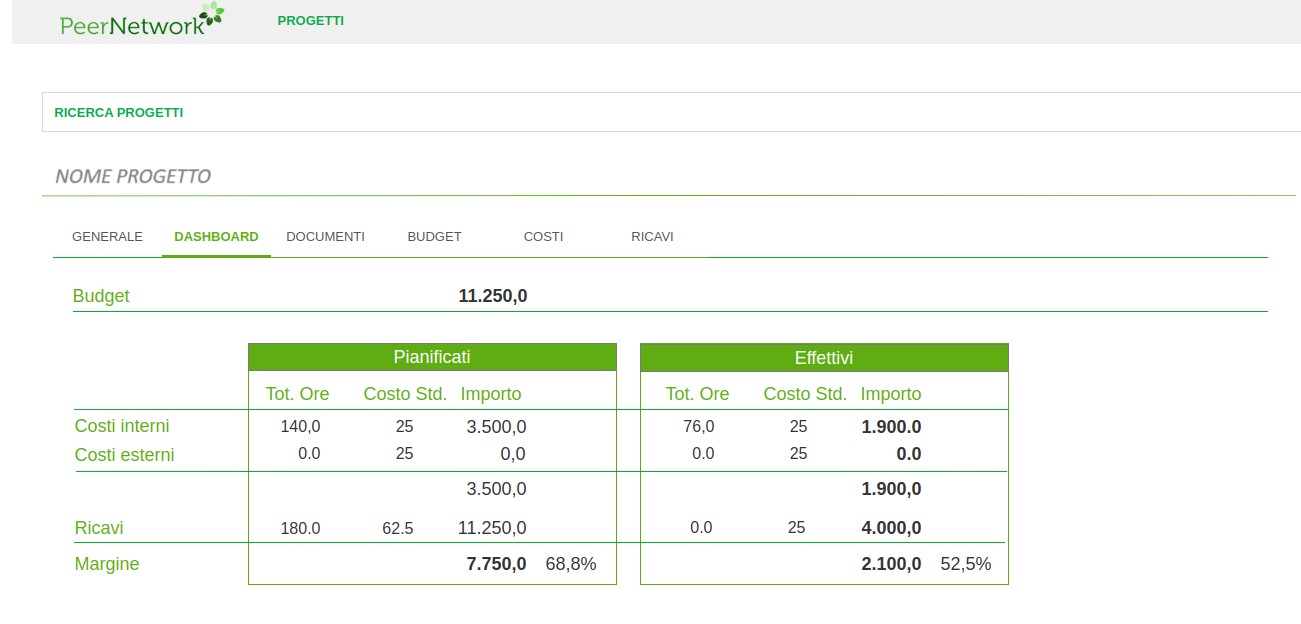
\includegraphics[width=\linewidth]{figures/pam-dashboard.png}
        \caption{Mockup esplicativo della dashboard richiesta}
        \label{fig:mockup-pam}
    \end{figure}

    Nell’area Progetti dell’applicativo \ac{PAM} sono raccolte tutte le informazioni relative
    ai progetti sviluppati. Per ciascuno di essi è disponibile un riepilogo dettagliato che include gli aspetti
    organizzativi, come la composizione del team, le tariffe orarie in base al ruolo, il budget assegnato
    e altri dati economici.

    Osservando il mockup in Figura \ref{fig:mockup-pam}, si nota che la sezione dedicata allo stato economico
    del progetto comprende costi, ricavi e margini, sia pianificati che reali. I valori previsionali
    vengono definiti all’inizio del progetto sulla base del budget disponibile concordato
    con il cliente, inserito nel sistema dal project manager. I dati effettivi, invece, si aggiornano in modo automatico.
    I tempi di lavoro vengono registrati dai dipendenti su Jira e poi sincronizzati in \ac{PAM} attraverso i \textbf{timeLog}.
    Un timeLog rappresenta una sessione di lavoro svolta da un utente su una specifica attività di un determinato progetto ed è caratterizzato da
    data, durata e descrizione dell’attività svolta. Oltre ai dati sui tempi di lavoro, il sistema integra anche le
    informazioni relative alle pre-fatture, che vengono generate dai project manager e dall’amministrazione all’inizio
    della fase di fatturazione.
    
    Per il recupero dei dati previsionali, viene utilizzata l’azione \texttt{projectGetDetails}, fornita dalla PBC 0801 PROJECT
    all’interno del GROUP G08 PROJECTS. Il budget di progetto rappresenta il valore economico totale assegnato ed è
    il punto di partenza per la definizione degli altri valori.

    In particolare, i \textbf{dati pianificati} vengono calcolati sulla base delle informazioni iniziali del progetto:
    \begin{itemize}
        \item costi interni: il totale delle ore viene determinato trasformando il numero di giornate a budget in ore e
        moltiplicando il risultato per un costo standard del dipendente;
        \item costi esterni: costi derivanti dall’impiego di risorse esterne, come le aziende partner. L’importo è dato
        dalla tariffa giornaliera concordata con il partner per il numero delle giornate assegnate alla risorsa;
        \item ricavi: l’importo corrisponde al budget assegnato al progetto, mentre il costo orario standard viene
        determinato in base al ruolo dei dipendenti coinvolti. La tariffa giornaliera dei dipendenti viene recuperata
        tramite l’azione \texttt{projectRateGetList} della PBC 0807 PROJECT RATE, appartenente al GROUP G08 PROJECTS. Il totale
        delle ore viene quindi calcolato dividendo il budget assegnato per la tariffa;
        \item margine: si ottiene come differenza tra l’importo dei ricavi e quello dei costi. La percentuale di margine
        viene calcolata rapportando questo valore rispetto ai ricavi complessivi.
    \end{itemize}

    I \textbf{dati effettivi}, invece, vengono aggiornati in tempo reale sulla base delle informazioni registrate nel sistema
    durante l’avanzamento del progetto:
    \begin{itemize}
        \item costi interni: il totale delle ore è dato dalla somma di tutte quelle effettivamente caricate dai
        dipendenti su Jira. Il recupero di questi dati avviene tramite l’azione timeLogGetList dalla PBC 0803 TIMELOG
        nel GROUP G08 PROJECTS, mentre costo standard e importo vengono ricalcolati secondo la stessa logica dei dati pianificati;
        \item costi esterni: costi derivanti dall’impiego di risorse esterne, come per i dati pianificati;
        \item ricavi: il valore è dato dalla somma di tutte le pre-fatture emesse per il progetto, estratte con l’azione
        \texttt{preInvoiceGetList}. Poiché la pre-fattura
        è un concetto specifico dell’applicativo \ac{PAM}, è stata adattata la PBC INVOICE del GROUP G16 1601 INVOICING,
        facendola diventare PAM PREINVOICE;
        \item margine: sia l’importo che la percentuale vengono calcolati secondo la stessa metodologia utilizzata per i dati pianificati.
    \end{itemize}

    \subsection{Aggiornamento database}
    Durante l'implementazione della dashboard riepilogativa dei dati economici di un progetto, è emerso un
    disallineamento nei totali delle pre-fatture visualizzate. Il problema è stato individuato confrontando
    i dati mostrati nella dashboard con quelli disponibili nell'area del portale denominata Attività Mensili,
    in particolare nella sezione che permette di visualizzare l’elenco completo delle pre-fatture associate a un cliente.
    Un'analisi approfondita ha evidenziato che l'incongruenza era dovuta a un disallineamento dei dati nel
    database. Nello specifico, per le prime pre-fatture generate tramite il portale a novembre 2024, il sistema
    non prevedeva ancora il salvataggio del progetto di riferimento, funzionalità introdotta solo nei mesi successivi.
    Per risolvere il problema, è stato necessario aggiornare i record incompleti direttamente in produzione tramite
    uno script MySQL. Lo script ha incrociato i dati di diverse tabelle del database per risalire ai valori corretti
    e garantire l'allineamento delle informazioni.

    \subsection{Modifiche nell'area Attività Mensili}
    Sono state apportate alcune modifiche per rendere l'area Attività Mensili più intuitiva ed efficiente.
    Questa sezione, già in uso, permette di monitorare e rendicontare mensilmente le ore di lavoro dei dipendenti
    sui vari progetti, oltre a generare automaticamente i report mensili da allegare alle fatture destinate ai
    clienti. Le principali modifiche grafiche introdotte sono state:
    \begin{itemize}
        \item l'inserimento di un form con input e pulsante di salvataggio: è stata aggiunta la possibilità di
        modificare alcuni campi della testata delle pre-fatture, come il numero AGO e il numero CRM, sia nella
        sezione Pre-fatture che in quella di Controllo Amministrazione. A tal fine, è stato introdotto un pulsante
        di salvataggio accanto a ogni pre-fattura modificabile;
        \item l'aggiunta di righe verticali per separare i campi: nella sezione riepilogativa delle Pre-fatture
        è stata implementata una riga divisoria tra le colonne dello specchietto riassuntivo, dove vengono
        visualizzati i totali del fatturato se le pre-fatture sono standard o manuali. Poiché il numero di
        colonne può variare dinamicamente, la riga viene mostrata solo se sono presenti almeno due colonne di valori;
        \item l'allineamento dei campi e riduzione dello spazio bianco: per migliorare la leggibilità dell’interfaccia,
        è stata ridotta la distanza tra i dati di testata della Pre-fattura, sia nella sezione Pre-fatture che in quella
        di Controllo Amministrazione.
    \end{itemize}

    Oltre ai cambiamenti grafici, sono state sviluppate logiche per garantire la correttezza di alcuni dati
    visualizzati e gestiti dall’applicativo, come:
    \begin{itemize}
        \item il salvataggio dei valori inseriti nel form: è stato implementato il meccanismo per permettere il salvataggio
        nel database dei valori AGO e CRM delle pre-fatture modificati dagli utenti. In questo modo, le informazioni
        aggiornate vengono conservate correttamente e rese disponibili per le successive elaborazioni;
        \item la correzione del calcolo dell’importo totale delle pre-fatture: nella sezione Controllo Amministrazione, è
        stato verificato e corretto il calcolo del totale da fatturare. Il problema risiedeva nel fatto che il sistema
        non considerava le pre-fatture manuali, ovvero quelle create dall’amministrazione ma che non
        derivano dal flusso standard di conferma delle ore in Jira. Ora il riepilogo tiene conto di entrambe le tipologie
        di pre-fatture, sia quelle standard che quelle manuali;
        \item l'assegnazione corretta del creatore di ogni pre-fattura: nelle sezioni Controllo Amministrazione e Pre-fatture,
        il campo relativo al project manager responsabile della pre-fattura non veniva correttamente visualizzato.
        Il problema è stato risolto implementando un meccanismo di recupero del project
        manager corretto per ogni pre-fattura, garantendo la corretta associazione dei dati.
    \end{itemize}

\chapter{Risultati}
\label{chap:Results}

In questo capitolo vengono illustrati i risultati ottenuti. Per quanto riguarda il miglioramento
della gestione dei progetti, vengono presentate le soluzioni proposte e accettate dalla direzione,
mirate a rendere il lavoro più efficiente. Per quanto riguarda lo sviluppo dell’applicativo \ac{PAM},
invece, si riporta l’interfaccia principale realizzata, fornendo una visione chiara del contributo
pratico apportato.

\section{Gestione Progetti}
Sulla base delle proposte illustrate nel Capitolo \ref{chap:pm}, la direzione e il responsabile dei
project manager hanno concordato di rendere immediatamente obbligatorie alcune pratiche in ogni fase
del ciclo di vita di un progetto, applicandole sin da subito ai nuovi progetti.
La decisione è stata accolta positivamente da tutti i dipendenti, con la volontà comune di allinearsi per migliorare
la qualità del lavoro, riconoscendo l’utilità e l’applicabilità immediata delle soluzioni individuate.
Le azioni descritte di seguito, suddivise per ciascuna fase progettuale, rappresentano quelle maggiormente adattate
alle esigenze aziendali. Partendo dalle proposte iniziali, sono state perfezionate attraverso un confronto diretto
con la direzione e i project manager, garantendone una migliore integrazione nel contesto operativo.

    \subsection{Idea, Design, Economics}
    Nella fase iniziale, quando il progetto non è ancora confermato e l'obiettivo è valutare il potenziale interesse
    del cliente, verranno svolte una serie di \textbf{riunioni esplorative con il committente}.
    Dal momento che in azineda non è presente una figura commerciale, durante gli incontri sarà il CEO ad occuparsi
    di convincere il cliente ad acquistare un nuovo sistema. Le conversazioni
    possono includere la visione di alcuni mockup o presentazioni per dare un'idea preliminare delle soluzioni realizzabili.

    Quando un cliente decide di avviare un nuovo progetto, viene assegnato un project manager di riferimento.
    Per garantire un \textbf{allineamento} iniziale efficace, si svolge un breve incontro \textbf{tra il CEO e il project manager},
    durante il quale il primo fornisce il contesto del progetto in modo informale.
    Questo confronto permette di chiarire gli obiettivi e definire una base solida per la gestione complessiva.

    Successivamente si passa a \textbf{incontri più strutturati con il cliente} per approfondire le idee, definire gli obiettivi
    e individuare le aree di maggiore interesse. A queste riunioni di approfondimento partecipano sia il CEO che il project
    manager, utilizzando mockup più dettagliati per affinare le specifiche e garantire una visione chiara del progetto.

    Man mano che si svolgono le riunioni, le informazioni raccolte vengono inserite e aggiornate nei documenti Confluence,
    con particolare attenzione ai \textbf{requisiti funzionali e non funzionali}. Questa attività viene svolta
    congiuntamente dal CEO e dal project manager, garantendo una documentazione chiara e sempre aggiornata.

    \subsection{Progetto Software}
    \subsubsection{Avvio}

    Subito dopo aver concordato con il cliente le specifiche del progetto, viene individuata la persona responsabile
    della gestione operativa, il \textbf{team leader}, il quale ha il compito di coordinare le attività tecniche di sviluppo.

    Tutti i \textbf{documenti} prodotti nelle fasi precedenti vengono \textbf{condivisi} al team leader, permettendogli di
    acquisire una visione chiara del progetto prima dell’inizio delle attività operative.

    Dopodiché, si organizza una \textbf{riunione di allineamento interna} rapida (massimo tenta minuti) tra il team leader,
    project manager e CEO, così da chiarire eventuali dubbi emersi dopo l’analisi della documentazione e definire gli aspetti principali del progetto.

    In incontri successivi, il project manager e il team leader \textbf{analizzano i rischi} suddividendoli in diverse categorie: tecnici,
    di project management, organizzativi ed esterni. Per quelli legati alla sicurezza informatica, si utilizza il modello STRIDE illustrato precedentemente.
    L’impatto e la probabilità di ogni rischio vengono classificati attraverso la matrice di rischio, suddivisa nei tre livelli: basso, medio e alto.

    Per quanto riguarda la \textbf{definizione delle risorse umane necessarie}, si identificano sin da subito le figure professionali richieste
    per lo sviluppo del progetto. Ad esempio, se tutte le \ac{PBC} necessarie sono
    già disponibili, potrebbero servire solo sviluppatori frontend per implementare l’interfaccia grafica, senza necessità di risorse backend.
    
    \subsubsection{Pianificazione}
    La suddivisione del lavoro in attività e sottoattività a livello logico deve essere organizzata in una \textbf{\ac{WBS}} ad albero,
    utilizzando una lavagna condivisa su \textbf{Miro}. Questo permette una visualizzazione chiara della struttura del progetto e
    facilita la collaborazione tra i membri del team.

    Per la \textbf{pianificazione} ad alto livello di progetto sarà obbligatorio creare un \textbf{Gantt} con l’utilizzo di GanttPRO.
    Questo strumento consente di definire una pianificazione temporale dettagliata, individuando le dipendenze tra le attività.
    Il piano deve essere condiviso e aggiornato con il cliente.

    Per garantire una gestione ordinata ed efficace del progetto, è fondamentale attenersi alle linee guida definite per
    la \textbf{pianificazione e progettazione su Jira}. Epic, task e subtask devono essere strutturati in modo coerente,
    partendo dalla \ac{WBS} e rispettando la gerarchia indicata. Il project manager sarà responsabile della definizione di epic e task,
    mentre il team leader si occuperà di dettagliare le attività tecniche operative attraverso la creazione dei subtask.

    \subsubsection{Esecuzione}
    Per definire standard aziendali condivisi, i quali servono a garantire coerenza e qualità nel lavoro di tutti, sarà necessario
    svolgere una \textbf{riunione sulle linee guida per gli sviluppatori} il prima possibile, nella quale si parlerà di:
    \begin{itemize}
        \item \textbf{convenzioni tecniche}, tra cui la nomenclatura di commit, branch e altre pratiche di versione del codice;
        \item \textbf{documentazione del codice}, con particolare attenzione alla spiegazione delle logiche complesse adottate;
        \item aggiornamento costante della \textbf{documentazione di progetto}, includendo qualsiasi modifica significativa,
        ad esempio il cambiamento della struttura dati di una \ac{PBC}.
    \end{itemize}

    Alla fine di ogni giornata lavorativa, è essenziale \textbf{aggiornare i subtask} su cui si è lavorato. Oltre a
    registrare le ore impiegate, ciascun dipendente deve modificare lo stato di avanzamento dei compiti svolti e aggiungere
    un riepilogo delle attività svolte nella sezione relativa ai commenti, oltre a eventuali difficoltà riscontrate.
    
    Tutte le \textbf{scadenze e i rilasci} significativi devono essere inseriti nel documento riepilogativo aziendale
    dello stato di tutti i progetti. Questo facilita il monitoraggio da parte del responsabile dei project manager e della direzione,
    garantendo una visione chiara dell’andamento generale.

    \subsubsection{Rilascio}
    Dopo ogni rilascio significativo, si organizza una \textbf{riunione retrospettiva interna} con tutto il team di progetto. Questo momento
    di confronto permette di evidenziare sia gli aspetti positivi, rafforzando la motivazione, soprattutto per i membri meno
    esperti, sia quelli negativi, offrendo spunti di miglioramento per il futuro.

\begin{figure}
    \centering
    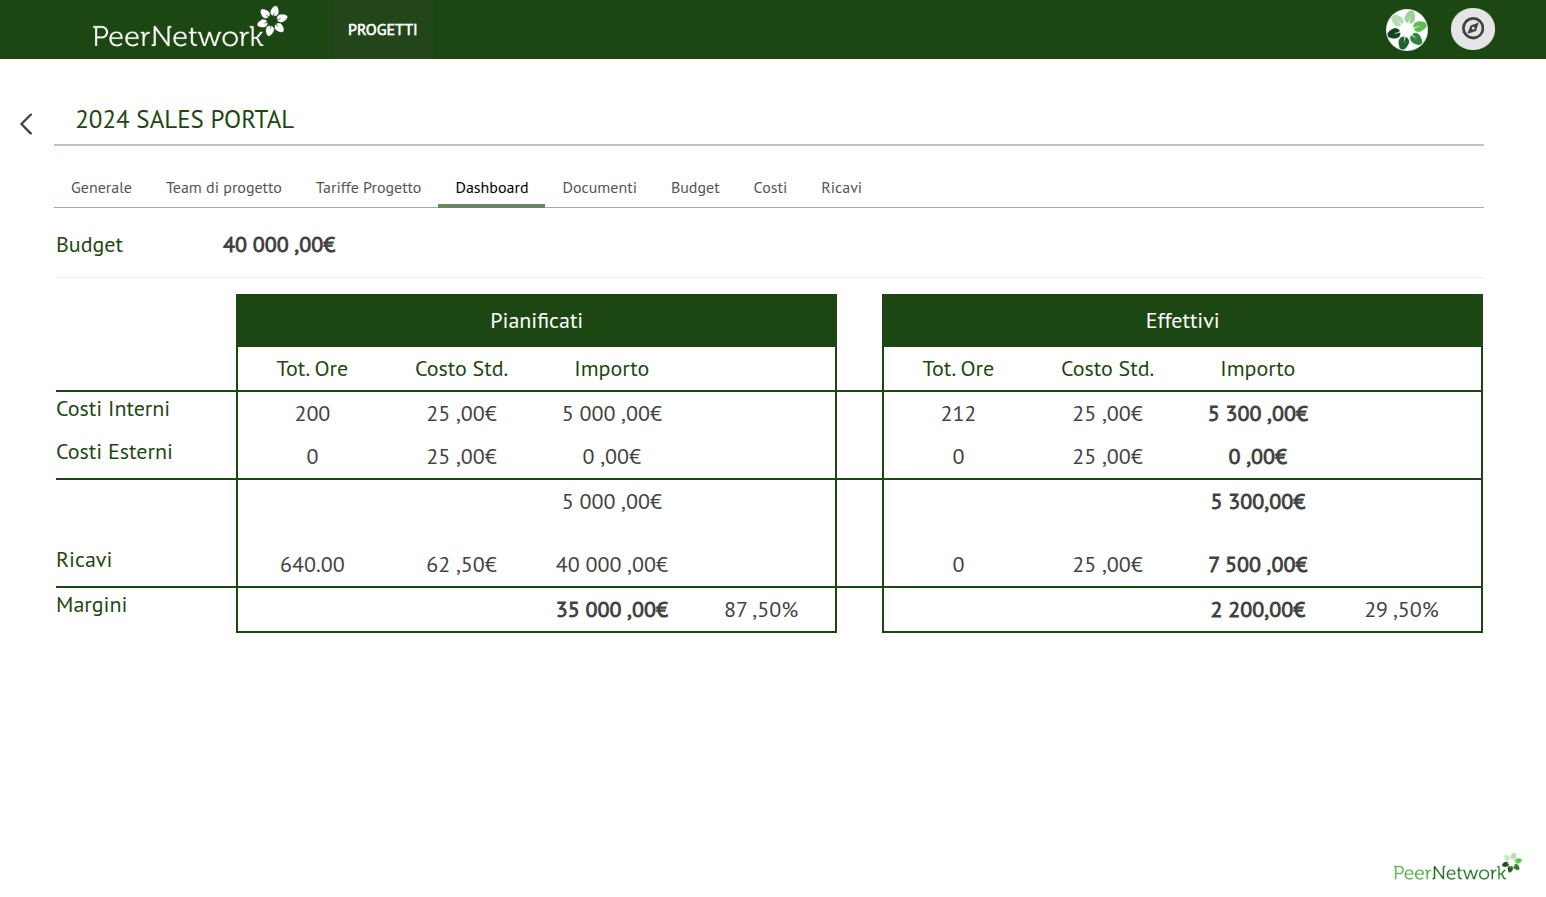
\includegraphics[width=\linewidth]{figures/dashboardPAM.png}
    \caption{Dashboard riepilogativa dei dati economici di un progetto}
    \label{fig:pam-dashboard}
\end{figure}
\section{Peer Network Activity Management}
Nell'area Progetti dell’applicazione \ac{PAM}, ogni progetto gestito dall’azienda dispone di una sezione dedicata
contenente tutte le informazioni rilevanti.
Come mostrato in Figura \ref{fig:pam-dashboard}, i dati specifici del progetto sono organizzati in diverse categorie:
informazioni generali (contenenti ad esempio cliente, budget e scadenze), composizione del team, tariffe di progetto
(costo giornaliero per dipendente in base al ruolo), oltre a riepiloghi economici e documenti (come le pre-fatture emesse).
In particolare, l'immagine riporta l'interfaccia principale sviluppata, attualmente già in uso dalla direzione e
dall'area amministrativa, denominata dashboard. Per motivi di riservatezza, la schermata presenta dati fittizi relativi
a un progetto simulato.

Basandosi sul mockup e sulle funzionalità richieste illustrate nel Capitolo \ref{chap:pam}, l’interfaccia permette
di visualizzare costi, ricavi e margini, sia pianificati che effettivi.
Alcuni valori pianificati, come il budget (indicato anche come importo del ricavo previsto) e le ore considerate
come costo interno, vengono inseriti dal project manager nella sezione riguardo le informazioni generali
del progetto, descritta in precedenza.
Il costo standard, utilizzato per il calcolo dei ricavi, si basa sulle tariffe di progetto, definite manualmente all’inizio del
progetto nella rispettiva sezione.
Gli altri valori previsionali vengono invece determinati attraverso semplici calcoli basati sui dati già disponibili.
I valori reali, invece, si aggiornano automaticamente: i costi effettivi vengono calcolati in base alle ore di lavoro
registrate dai dipendenti su Jira, mentre i ricavi effettivi derivano dalla somma delle pre-fatture emesse mensilmente al cliente.

\chapter{Conclusioni e Sviluppi Futuri}

%(1) Briefly recall problem, starting point and methods adopted,
%(2) Briefly report Findings,
%(3) Briefly discuss benefits/limitations,
%(4) Discuss Future Work

Lo scopo del lavoro svolto è stato ottimizzare la gestione dei progetti aziendali della \textit{Peer Network}.
Per proporre soluzioni concrete, introducendo nuove attività o modificandone alcune esistenti, è stato
innanzitutto necessario analizzare a fondo il processo attuale, dall’iniziale contatto con il cliente
fino all’installazione completa della soluzione e al successivo servizio di supporto. In un secondo momento,
attraverso un confronto con la direzione e i project manager, sono state selezionate alcune proposte
da implementare. Parallelamente, sono state svolte attività di sviluppo nell’applicativo interno \ac{PAM}.
Oltre a piccoli interventi sul frontend, il contributo principale ha riguardato la realizzazione
dell’interfaccia grafica, con la relativa logica, per il riepilogo dei dati economici di ciascun
progetto, consentendo la visualizzazione di costi, ricavi e margini sia pianificati che effettivi.

Per valutare l’efficacia delle soluzioni adottate e il loro impatto in termini di risparmio
di tempo e miglioramento della qualità del lavoro svolto, è essenziale che l’azienda le applichi in
modo sistematico. Solo dopo alcuni mesi, una volta consolidate come prassi operative per tutti i dipendenti,
sarà possibile effettuare un confronto significativo con i progetti precedenti.
Poiché al momento non è possibile un’analisi comparativa diretta, data la necessità di un periodo di
assestamento, un’alternativa potrebbe essere il monitoraggio progressivo delle nuove metodologie.
In particolare, misurare il tempo impiegato dalle risorse per svolgere specifiche attività prima e
dopo l’introduzione delle nuove pratiche permetterebbe di raccogliere dati concreti sul loro impatto.

Per quanto riguarda \ac{PAM}, un’evoluzione naturale del sistema consisterebbe nell’integrare al suo
interno tutte le funzionalità attualmente gestite tramite fogli elettronici o altri strumenti esterni,
trasformandolo a tutti gli effetti in un sistema informativo aziendale.
Partendo dall’interfaccia sviluppata, focalizzata sulla gestione dei dati economici di progetto, si
potrebbe ampliare il sistema includendo una sezione dedicata al monitoraggio di ricavi e costi,
sia pianificati che reali, su base mensile. I dati previsionali, solitamente inseriti dal project manager
in un foglio elettronico, verrebbero direttamente registrati nell’applicativo, consentendo l’introduzione
di strumenti avanzati di analisi, come grafici e statistiche sulle proiezioni finanziarie.
Una volta integrati tutti questi elementi, si potrebbe sviluppare un’area riservata alla direzione e
all’amministrazione aziendale, dedicata all’analisi economica complessiva. Questa sezione offrirebbe
statistiche mensili e annuali su ricavi, costi e margini aziendali, sintetizzando le informazioni già
in possesso. Un simile strumento risulterebbe estremamente utile per monitorare l’andamento economico
della \textit{Peer Network} e supportare decisioni strategiche su investimenti in nuove risorse,
attrezzature e aggiornamenti.

%----------------------------------------------------------------------------------------
% BIBLIOGRAPHY
%----------------------------------------------------------------------------------------

\backmatter

\nocite{*} % Remove this as soon as you have the first citation

\bibliographystyle{alpha}
\bibliography{bibliography}

%\begin{acknowledgements} % this is optional
%Optional. Max 1 page.
%\end{acknowledgements}

\end{document}
